\documentclass[11pt,a4paper]{article}

% ----------------------------------------------------------------------
% Living draft of the methods paper:
%   "Radiative-transfer correction of Herschel-derived prestellar
%    core masses: a bias-vs-environment framework for Aquila"
%
% Written as a working document to preserve the method definition and,
% especially, the validity / scope reasoning while the model grid is
% being built. Portable article class so it compiles anywhere; can be
% switched to aa.cls for A&A submission later.
% ----------------------------------------------------------------------

\usepackage[T1]{fontenc}
\usepackage{amsmath,amssymb}
\usepackage{graphicx}
\usepackage{geometry}
\geometry{margin=2.4cm}
\usepackage[expansion=false]{microtype}
\usepackage[round,authoryear]{natbib}

% AAS/A&A journal abbreviation macros (provided natively by aa.cls;
% defined here for portable compilation with the article class)
\newcommand{\aap}{A\&A}
\newcommand{\aapr}{A\&ARv}
\newcommand{\apj}{ApJ}
\newcommand{\apjl}{ApJL}
\newcommand{\apjs}{ApJS}
\newcommand{\mnras}{MNRAS}
\newcommand{\araa}{ARA\&A}
\newcommand{\pasp}{PASP}
\newcommand{\qjras}{QJRAS}
\newcommand{\nat}{Nature}
\usepackage{xcolor}
\usepackage[hidelinks]{hyperref}

% editorial note macro
\newcommand{\note}[1]{\textcolor{magenta}{\textbf{[#1]}}}
\newcommand{\todo}[1]{\textcolor{red}{\textsf{TODO: #1}}}

\newcommand{\msun}{M_{\odot}}
\newcommand{\rhoc}{\rho_{\mathrm{c}}}
\newcommand{\cs}{c_{\mathrm{s}}}
\newcommand{\rzero}{r_{0}}
\newcommand{\Rbe}{R_{\mathrm{BE}}}
\newcommand{\Tbe}{T_{\mathrm{BE}}}
\newcommand{\ximax}{\xi_{\mathrm{max}}}
\newcommand{\Scloud}{\Sigma_{\mathrm{cloud}}}
\newcommand{\rhocloud}{\rho_{\mathrm{cloud}}}
\newcommand{\Rcloud}{R_{\mathrm{cloud}}}
\newcommand{\mH}{m_{\mathrm{H}}}
\newcommand{\Tsed}{T_{\mathrm{SED}}}

\title{\bfseries Radiative-transfer correction of Herschel-derived
prestellar core masses:\\ a bias--vs--environment framework}
\author{A.\ Men'shchikov, G.\ Zhang \note{author list/order TBD}}
\date{Working draft --- \today}

\begin{document}
\maketitle

\begin{abstract}
\noindent
Prestellar core masses derived from \emph{Herschel} dust continuum by
isothermal modified-blackbody (MBB) fitting of spectral energy
distributions (SEDs) are systematically biased. Two distinct physical
mechanisms drive the bias, and both act in the same direction
(mass under-estimation): (i)~internal temperature gradients make the
SED-weighted dust temperature warmer than the mass-weighted temperature
for centrally concentrated, externally heated cores, so the MBB fit
over-estimates the temperature and under-estimates the mass; and
(ii)~interpolated background subtraction over-subtracts flux for low-mass
cores, because the true cloud column under the core (the ``crater'')
is lower than the column interpolated from the surrounding edge.
We present a per-core radiative-transfer (RT) forward-modeling method
that reproduces the full observational chain
(RT imaging of the embedded core~$\rightarrow$~background
determination~$\rightarrow$~background subtraction) and recovers accurate
masses and temperatures by fitting
Bonnor--Ebert (BE) sphere models, parameterized by the observed mass and
size at a self-consistent temperature, to the observed
wavelength-dependent contrasts and sizes. The central deliverable is a
quantitative map of the mass bias as a function of core mass and cloud
column density. This document defines the method, records the
construction and calibration choices, and---at length---delimits the
regime of validity and the assumptions, with the tests that justify them.
\end{abstract}

% ======================================================================
\section{Introduction}
% ======================================================================

Dust continuum surveys with \emph{Herschel} have produced large catalogues
of dense cores and the prestellar core mass function (CMF), which is
widely compared to the stellar initial mass function. The masses underlying
these catalogues are obtained by fitting an isothermal MBB to the
background-subtracted SED of each extracted source. Both ingredients of
that procedure---the assumption of a single dust temperature and the
background subtraction---introduce systematic errors that propagate into
the derived masses and hence into the CMF.

The isothermal assumption fails because real cores are not isothermal:
externally heated, centrally concentrated cores are colder in the center
than at the surface. The SED of such a core is dominated by the warmer
outer layers, so the temperature recovered by an isothermal MBB fit
exceeds the mass-weighted temperature. Since the inferred mass scales as
$M \propto F_\nu / B_\nu(T)$, an over-estimated temperature yields an
under-estimated mass. This is the \emph{temperature-gradient warm bias};
it grows with central concentration and is largest for the more massive,
denser cores.

The background subtraction fails in a different regime. Standard pipelines
estimate the background under a source by interpolating the surrounding
emission across the source footprint. But an embedded core \emph{displaces}
the cloud material it occupies, so the cloud column directly behind the core
is lower than the column just outside it; the interpolated background
therefore over-estimates what should be subtracted and removes part of the
core's own flux. This \emph{over-subtraction flux loss} is most severe for
low-mass cores, whose own emission is comparable to the background.

The two mechanisms have different physical origins but push the recovered
mass the same way, so they compound rather than cancel. The method
described here corrects both simultaneously, because a forward RT model
that embeds a core in a cloud and applies the same background subtraction
as the observations reproduces both effects by construction. Rather than
using RT to populate backgrounds for completeness simulations, we compute
an RT model \emph{per extracted core} and fit it to the observed
band-dependent contrasts and sizes, recovering the mass and temperature
free of the MBB bias.

The product of the method is not a single corrected mass but a
\emph{bias-vs-environment surface}: the mass under-estimation as a function
of core mass and cloud column density. We develop and illustrate the method
on the Aquila star-forming region, for which a published core catalogue exists \citep{Konyves+2015}, with application to additional clouds deferred to a companion paper.

% ======================================================================
\section{Method}
% ======================================================================

\subsection{Overview}

For each core we forward-model the observable signal: a Bonnor--Ebert sphere
embedded in a uniform cloud, processed through Monte-Carlo dust RT
(RADMC-3D), projected, convolved to the \emph{Herschel} beams, resampled to
a common angular grid, and background-subtracted exactly as in the
observational reduction. Each model is specified by the core mass $M$ and its
size (intrinsic FWHM), which fix the truncation $\ximax$ and central density
through the inversion of Sect.~\ref{sec:inversion}; the construction
temperature $\Tbe$ is not free but is set self-consistently from the total
central shielding column (Sect.~\ref{sec:tbe}), and the local cloud column
$\Scloud$ is supplied per core from the observed background. The fit minimizes
the residual between modeled and observed band-dependent center intensities and
FWHMs. Completeness is treated separately (via source extraction with getsf,
\citealp{Menshchikov2021method}) and is not part of the mass-accuracy chain.

\subsection{The Bonnor--Ebert sphere model family}

We adopt critical isothermal Bonnor--Ebert spheres \citep{Ebert1955,Bonnor1956}
as the core density-profile template. The dimensionless density $e^{-\psi(\xi)}$ follows the
isothermal Lane--Emden equation
\begin{equation}
  \frac{1}{\xi^{2}}\frac{\mathrm{d}}{\mathrm{d}\xi}
  \!\left(\xi^{2}\frac{\mathrm{d}\psi}{\mathrm{d}\xi}\right)
  = e^{-\psi},
  \qquad \psi(0)=0,\ \ \psi'(0)=0,
  \label{eq:lane-emden}
\end{equation}
with $\rho(\xi)=\rhoc\,e^{-\psi(\xi)}$ and the physical radius
$r=\xi\,\rzero$, where the scale length is
\begin{equation}
  \rzero = \frac{\cs}{\sqrt{4\pi G \rhoc}},
  \qquad
  \cs^{2} = \frac{k_{\mathrm B}\,\Tbe}{\mu_{\mathrm p}\,\mH}.
  \label{eq:r0}
\end{equation}
A single model is specified by three numbers: the isothermal temperature
$\Tbe$ (through $\cs$), the central density $\rhoc$, and the dimensionless
truncation radius $\ximax$ at which the sphere is cut and joined to the
surrounding cloud. Earlier versions of this work fixed $\ximax = 6.451$, the
critical value at which the center-to-edge contrast is
$\rhoc/\rho(\ximax) = 14.0$ and the sphere is marginally stable. We no longer
fix it. Instead $\ximax$ is a genuine construction variable that runs from
weakly concentrated, nearly uniform spheres ($\ximax \lesssim 1$), through the
critical value, to strongly concentrated super-critical profiles
($\ximax > 6.451$). The failure of the fixed-critical choice, and the physical
meaning of the sub-critical, critical, and super-critical regimes, are set out
in Sect.~\ref{sec:geometry}. The essential point for the method is that
$\ximax$ carries \emph{all} of the profile-shape information, while $\Tbe$ and
$\rhoc$ set only the physical scale; the family therefore has one shape
parameter ($\ximax$) and two scale parameters ($\Tbe$, $\rhoc$).

Three dimensionless shape functions, each a function of $\ximax$ alone,
summarize the family and are tabulated once from the solution of
Eq.~(\ref{eq:lane-emden}). The first is the enclosed-mass function $C(\ximax)$
defined in Eq.~(\ref{eq:Cxi}) below. The second is the center-to-edge density
contrast
\begin{equation}
  \mathcal{C}_{\rho}(\ximax) \equiv e^{\psi(\ximax)}
  = \frac{\rhoc}{\rho(\Rbe)} ,
  \label{eq:contrast}
\end{equation}
which grows from unity (uniform sphere) through $14.0$ at the critical radius
and continues to rise for super-critical truncations. The third is the
projected half-maximum width $\phi(\ximax)$, defined as the FWHM of the
line-of-sight column-density profile (the Abel projection of $e^{-\psi}$)
expressed in units of the scale length $\rzero$, so that the intrinsic
projected FWHM of a model is
\begin{equation}
  \mathrm{FWHM}_{\mathrm{intr}} = \phi(\ximax)\,\rzero .
  \label{eq:phidef}
\end{equation}
A useful and, at first, surprising property of $\phi$ is that it \emph{saturates}
at large $\ximax$ (it approaches $\phi \simeq 6.6$ as $\ximax \to \infty$): the
projected FWHM is fixed by the inner, nearly flat core and is almost
independent of how far the outer envelope is truncated. This saturation
controls the behavior of the compact, massive end of the grid
(Sect.~\ref{sec:grid}) and the resolution limit discussed there.

\subsection{Analytic central density and mass}
\label{sec:inversion}

A critical point of method construction is that the central density must be
derived from BE physics, \emph{not} imposed by renormalizing the profile to
a target mass. Renormalization produces incorrect central densities and
breaks code-to-code comparability. The enclosed dimensionless mass follows
from the first integral of Eq.~(\ref{eq:lane-emden}),
\begin{equation}
  C(\xi)\equiv\int_{0}^{\xi} e^{-\psi(\xi')}\,\xi'^{2}\,\mathrm{d}\xi'
  = \xi^{2}\,\psi'(\xi),
  \label{eq:Cxi}
\end{equation}
so the total mass of the truncated sphere is
\begin{equation}
  M = 4\pi\,\rhoc\,\rzero^{3}\,C(\ximax)
    = \frac{m_{1}}{\sqrt{4\pi}}\,
      \frac{\cs^{3}}{G^{3/2}\,\rhoc^{1/2}},
  \qquad
  m_{1}\equiv C(\ximax).
  \label{eq:mass}
\end{equation}
We evaluate $C(\xi)$ on our tabulated BE solution by the trapezoidal rule.
When the truncation was fixed at the critical radius, $C$ was a single number,
$C(6.451)=15.7086$, and Eq.~(\ref{eq:mass}) inverted directly to
$\rhoc=(4.4313\,\cs^{3}/G^{3/2}M)^{2}$ for a target mass at fixed $\Tbe$. With
$\ximax$ now free, $C$ varies from model to model and the inversion is a
two-step procedure driven by the two observables that define a core, its mass
$M$ and its size.

We specify each model by a target mass $M$ and a target intrinsic projected
width $\mathrm{FWHM}_{\mathrm{intr}}$ at a given $\Tbe$. Eliminating $\rhoc$ and
$\rzero$ between the mass relation, Eq.~(\ref{eq:mass}), and the width
definition, Eq.~(\ref{eq:phidef}), gives a single equation for the truncation
radius,
\begin{equation}
  \frac{\phi(\ximax)}{C(\ximax)}
  = \frac{\mathrm{FWHM}_{\mathrm{intr}}\,\cs^{2}}{M\,G} .
  \label{eq:xiinvert}
\end{equation}
The ratio $\phi/C$ is strictly monotone decreasing in $\ximax$, so
Eq.~(\ref{eq:xiinvert}) has a unique root: a core's mass and size together fix
its concentration, and hence $\ximax$. In physical terms $\ximax$ is tied to
the mass-to-size ratio and is not a free choice. Having solved for $\ximax$,
the scale length and central density follow in closed form,
\begin{equation}
  \rzero = \frac{M\,G}{\cs^{2}\,C(\ximax)},
  \qquad
  \rhoc = \frac{\cs^{2}}{4\pi G\,\rzero^{2}},
  \label{eq:rho_from_MFW}
\end{equation}
and the outer (truncation) radius is $\Rbe=\ximax\,\rzero$. We tabulate
$C(\xi)$ and $\phi(\xi)$ from the same BE solution used to build the profile,
so the inversion and the discretized profile remain mutually consistent.
\note{The single self-consistency point below was the source of an early
factor-$\sim$2 mass error: keep the inversion, the width function, and the
profile builder tied to one tabulated $\psi(\xi)$.}

Two properties of Eq.~(\ref{eq:xiinvert}) matter downstream. First, because
$\phi$ saturates at large $\ximax$ while $C \propto 2\ximax$ grows without
bound, the right-hand side can be made arbitrarily small only by driving
$\ximax$ very large; a massive core at a near-beam size therefore maps to a
very high concentration, and a genuinely unresolved core
($\mathrm{FWHM}_{\mathrm{intr}} \to 0$) would need $\ximax \to \infty$. This
sets a natural upper bound on the useful grid (Sect.~\ref{sec:grid}). Second,
raising $\Tbe$ at fixed $(M,\mathrm{FWHM})$ raises the right-hand side and so
lowers $\ximax$; the temperature used to build a model changes the shape
assigned to a given observed core, which is why the temperature must itself be
fixed on physical grounds (Sect.~\ref{sec:tbe}).

\subsection{Molecular-weight conventions}
\label{sec:mu}

Two distinct mean molecular weights enter, and conflating them is a common
error:
\begin{itemize}
  \item the mean molecular weight \emph{per free particle},
        $\mu_{\mathrm p}=2.33$, appears in the sound speed
        (Eq.~\ref{eq:r0}) and hence throughout the BE structure, because
        the supporting pressure is set by the total particle number,
        $P=n_{\mathrm{tot}}k_{\mathrm B}T$;
  \item the mean molecular weight \emph{per hydrogen molecule},
        $\mu_{\mathrm{H_2}}=2.8$, appears only in number-density$\leftrightarrow$
        mass-density and column conversions, e.g.\
        $N = \Sigma/(\mu_{\mathrm{H_2}}\mH)$.
\end{itemize}
Using $\mu=2.8$ in the sound speed (as in some earlier code) under-estimates
$\cs$ and therefore $\Rbe$ and the mass at fixed $\rhoc$; the correct value
for the structure is $\mu_{\mathrm p}=2.33$.

\subsection{Mass-conserving discretization}
\label{sec:massconserv}

RADMC-3D treats each cell as uniform and computes its mass as
$\rho_{\mathrm{cell}}\times V_{\mathrm{cell}}$ with the exact spherical
shell volume. Point-sampling the BE profile at cell centers does not
conserve mass on a coarse grid (we measured a $\sim$9\% deficit). We instead
assign each cell its mass-conserving shell-average density, obtained
directly from $C(\xi)$:
\begin{equation}
  \rho_{\mathrm{cell}}
  = 3\,\rhoc\,
    \frac{C(\xi_{\mathrm{out}})-C(\xi_{\mathrm{in}})}
         {\xi_{\mathrm{out}}^{3}-\xi_{\mathrm{in}}^{3}},
  \label{eq:cellrho}
\end{equation}
where $\xi_{\mathrm{in}},\xi_{\mathrm{out}}$ are the cell \emph{walls} in
dimensionless units (the scale length $\rzero$ cancels). Because adjacent
cells share a wall, $C(\xi_{\mathrm{out}})$ of one cell equals
$C(\xi_{\mathrm{in}})$ of the next, and the summed mass telescopes,
\begin{equation}
  \sum_{\mathrm{cells}} \rho_{\mathrm{cell}}\,V_{\mathrm{cell}}
  = 4\pi\,\rhoc\,\rzero^{3}\,
    \big[\,C(\xi_{\mathrm{edge}})-C(\xi_{\mathrm{inner}})\,\big],
  \label{eq:telescope}
\end{equation}
which is independent of the number of zones. The mass is therefore exact
(to the accuracy of the single tabulated integral $C$) at any resolution,
so we may use $\sim$100 radial zones---chosen for photon statistics rather
than to over-resolve the flat BE center---without losing mass. With a
finely spaced table the trapezoidal evaluation of $C$ and the linear
interpolation of $C$ onto the cell walls are both negligible sources of
error.

\subsection{Grid construction and the continuity constraint}
\label{sec:continuity}

To eliminate the boundary cell that straddles $\Rbe$ (which otherwise
requires a fragile mixed BE/cloud treatment and breaks the telescoping
sum), we snap a radial wall exactly to $\Rbe$. Every cell is then
unambiguously pure BE (outer wall $\le \Rbe$) or pure cloud
(inner wall $\ge \Rbe$); no cell is partly both, the BE and cloud
assignment loops cannot disagree about a shared cell, and
Eq.~(\ref{eq:telescope}) holds exactly.

We further impose a physical/numerical self-consistency requirement on the
embedding: the core joins the cloud as an overdensity,
\begin{equation}
  \rho_{\mathrm{BE}}(\Rbe)\;\ge\;\rhocloud .
  \label{eq:contconstraint}
\end{equation}
In an earlier pipeline this was enforced as a hard constraint, because that
pipeline convolved the full core-plus-cloud image to the beam \emph{before}
subtracting the background: when the BE edge density fell below the cloud
density, the beam smeared the higher surrounding cloud inward and the
subsequent subtraction left a spurious negative feature---a depression rather
than a core. We have since changed the operation order: the constant cloud
pedestal is subtracted from the \emph{original} (unconvolved) model image, at
the local floor $\rho_{\mathrm{BE}}(\Rbe)$ rather than at the denser cloud
value, and only then is the isolated core excess convolved. Subtraction on the
original image is exact and linear, so no depression can form, and we have
verified on models spanning edge-to-cloud density ratios from $1.13$ down to
$0.08$ that the recovered mass is unbiased in every case
(Sect.~\ref{sec:cratervsinterp}). Equation~(\ref{eq:contconstraint}) is
therefore \emph{no longer imposed}: the models it once excluded---compact,
massive cores whose rarefied edge sits below the surrounding cloud---are
retained. Such an inner rarefaction relative to the ambient cloud is, in fact,
schematically what an inside-out collapsing core develops as material drains
inward behind the infall front, so these configurations plausibly represent
real evolved cores rather than an artefact to be excluded. The Monte-Carlo
radiative transfer handles the density inversion without difficulty: within
the depression photons propagate with fewer interactions, so the equilibrium
temperature neither spikes nor drops but varies smoothly across the boundary.

\subsection{Radiative transfer and the interstellar radiation field}
\label{sec:rt}

We use RADMC-3D \citep{Dullemond+2012}, a Monte-Carlo dust radiative-transfer
code, for the production grid. An earlier
ray-tracing code (\textsc{modust}) showed $\sim$10--20\% non-monotonic
intensity oscillations in the densest models and under-heated the interior
by $\sim$3~K; the latter is a converged physics/implementation limit in the
diffuse re-emission, not a convergence error, so we adopt RADMC-3D
throughout (the cross-validation is given in Sect.~\ref{sec:crossval}).

The heating field is the standard interstellar radiation field (ISRF),
tabulated as the Black field plus a scaled hot blackbody, normalized to
$G_{0}\approx 10$. The far-ultraviolet integral, taken with the
$4\pi$ solid angle, gives
$G_{0}=4\pi\times 1.22\times10^{-3}/1.6\times10^{-3}\approx 10$. The RT
computes the cloud temperature self-consistently for each model; $G_{0}$ is
held fixed (Sect.~\ref{sec:g0}). We omit the polycyclic aromatic
hydrocarbon (PAH) emission bands: adding them changes core-center
temperatures by only $\sim$1--2\% in the correct RT (diffuse re-emission
dominates the interior heating), and the apparent PAH dependence in
\textsc{modust} was compensating for its interior under-heating.

\subsection{Embedding cloud: variable radius and the $\Scloud$ axis}
\label{sec:cloud}

The core is embedded in a uniform-density sphere. The cloud radius must be
large enough that (i)~the beam never reaches the boundary and (ii)~there is
enough clean cloud around the core for the background estimate to behave as
in the real reductions. Both requirements scale with the \emph{convolved}
core size, so we size the cloud to the quadrature combination of the
beam and core scales,
\begin{equation}
  \Rcloud = f_{\mathrm{r}}\,
  \sqrt{(\theta_{500}\,d)^{2} + \Rbe^{2}},
  \label{eq:rcloud}
\end{equation}
with the largest \emph{Herschel} beam $\theta_{500}=36.3''$ (the worst
case, which covers all bands), distance $d$, and ratio $f_{\mathrm{r}}\approx
30$ (chosen so the projected cloud surface density is flat across the core
footprint and the background annulus). The truncation radius $\Rbe$ and the
beam half-width are comparable measures of width---a projected, convolved
critical-BE column is close to Gaussian, so its truncation radius is near
the Gaussian half-width---so adding them in quadrature combines like
quantities. Equation~(\ref{eq:rcloud}) reduces to beam-dominated for
unresolved cores (all such cores acquire the same physical cloud size) and
to core-dominated for resolved cores, with a smooth crossover and no kink.

Because $\Rcloud$ varies, the cloud's external shielding column---and hence
its temperature structure next to the core---would vary per model if
$\rhocloud$ were held fixed. The physically meaningful, model-invariant
quantity is the line-of-sight cloud column, not the volume density. We
therefore make the third grid axis the cloud surface density $\Scloud$
(measured along a sightline just outside the core, to avoid the
crater; Sect.~\ref{sec:bgdetermination}),
\begin{equation}
  \Scloud = \rhocloud\,\frac{2\sqrt{\Rcloud^{2}-\Rbe^{2}}}
                              {\mu_{\mathrm{H_2}}\mH}
  \quad\Longrightarrow\quad
  \rhocloud = \frac{\Scloud\,\mu_{\mathrm{H_2}}\mH}
                   {2\sqrt{\Rcloud^{2}-\Rbe^{2}}},
  \label{eq:sigmacloud}
\end{equation}
holding $\Scloud$ at fixed grid values and deriving $\rhocloud$ per model.
This recovers identical cloud RT at a given $\Scloud$ node across all masses,
matches the axis to the observed local background, and---together with the
revised background subtraction---removes the earlier need to trim on
Eq.~(\ref{eq:contconstraint}). The grid records $\Scloud$ (the axis) together
with the derived $\rhocloud$ and $\Rcloud$ (needed for reproducibility and for
the RT construction, both defined on $\rhocloud$).

\subsection{Background determination: crater versus interpolated}
\label{sec:bgdetermination}

The RT imaging produces the \emph{total} emergent intensity of the
embedded core in one self-consistent computation; the bias does not enter
there but in
how the cloud contribution under the source is subsequently determined and
subtracted. We implement two background schemes alongside each other:
\begin{itemize}
  \item the traditional \emph{interpolated} background, in which the
        cloud contribution under the source is interpolated across the
        source footprint from the surrounding cloud-only sightlines (a
        nearly flat estimate);
  \item the \emph{crater} background, computed from a \emph{second} RT run of
        the same cloud with the core density zeroed inside $\Rbe$ (the core
        physically removed, leaving a cavity). This gives the true,
        reduced cloud emission along the central sightline---lower than the
        surrounding cloud because the core has displaced the material that
        would otherwise lie behind it.
\end{itemize}
We use ``crater'' as the running term because it describes the background
\emph{shape} compactly and visually (a central depression with a raised
rim); it is the same feature termed ``limb-brightened'' in earlier work,
which names the corresponding intensity signature (the projected rim of the
cavity is brighter than its center). The interpolated background, blind to
the crater, over-estimates the cloud contribution under the core, so its
subtraction removes part of the core's own flux. The contrast between the
two schemes is the direct measure of the over-subtraction flux loss
(Sect.~\ref{sec:cratervsinterp}).

\subsection{Observables}
\label{sec:observables}

For each model we measure, on the beam-convolved, resampled, background-
subtracted image, the signed center (peak) intensity (the contrast) and the
FWHM, at the surface-density map (\texttt{SD}) and at each of the five
\emph{Herschel} bands (70, 160, 250, 350, 500\,$\mu$m), up to twelve
observables per core. Two choices matter:
\begin{itemize}
  \item the band-dependent FWHM is the temperature-gradient diagnostic
        (a colder center is more centrally concentrated at the longer
        wavelengths);
  \item the \emph{signed} center intensity (not the peak) handles
        donut/absorption morphology: the 70\,$\mu$m center intensity is
        physically negative for cold cores seen in absorption, and this
        sign carries information.
\end{itemize}
\note{\texttt{SD} (surface density) is a different kind of observable from
the band intensities---different units and noise model---so its
$\sigma$-normalization in the fit must be set accordingly and it must not be
weighted as a flux.}

\subsection{The recovered-concentration observable}
\label{sec:concentration}

A third observable is needed once the grid is expressed in terms of the mass
that \emph{getsf} actually recovers rather than the model's true mass
(Sect.~\ref{sec:recoverable}). The recoverable-mass transform is not
monotonic in $M_{\mathrm{BE}}$: at fixed cloud column the coldest, lowest-
density cores lose so large a flux fraction to cirrus confusion that a
higher-mass cold core can recover \emph{less} mass than a lower-mass warmer
one. Recovered mass and cloud column alone are therefore insufficient to
invert the correction near this fold. The degeneracy is broken by a
concentration observable---the ratio of the source footprint size to its
FWHM---which is systematically larger for a compact core than for the
partially recovered central region of an over-resolved diffuse core. We adopt
the footprint-to-FWHM ratio on the surface-density map ($\mathrm{FOOA}/
\mathrm{AFWHM}$ at the $161\,\mu$m column-density band in the \emph{getsf}
catalogue), which is measured identically in the grid and in the extraction
and so enters the interpolation without a unit or definition mismatch. The
correction interpolant is thus three-dimensional: recovered mass, cloud
column $\Scloud$, and this concentration ratio.
\note{The validated \texttt{RecoverableCorrector} uses a fourth axis, the
source FWHM on the $161\,\mu$m band, alongside the concentration ratio.
Promote this paragraph to a four-dimensional interpolant to match the code;
Sect.~\ref{sec:geometry} already invokes the four-observable set (recovered
mass, $\Scloud$, source FWHM, concentration) and explains why neither the
recovered mass nor the concentration is redundant.}

\subsection{Construction temperature and self-consistency}
\label{sec:tbe}

The temperature $\Tbe$ that enters the inversion, Eq.~(\ref{eq:xiinvert}), is the
isothermal temperature at which the hydrostatic profile is built. It must be kept
distinct from the dust temperature structure $T_{\mathrm{dust}}(r)$ that RADMC-3D
computes for that profile: the latter is not isothermal, and it carries the
warm-envelope, cold-center gradient that drives the mass bias this paper corrects.
The construction temperature sets the profile scale, but through
Eq.~(\ref{eq:xiinvert}) it also fixes the shape ($\ximax$) assigned to a given
observed $(M,\mathrm{FWHM})$, so it cannot be chosen arbitrarily. We take $\Tbe$
to be the mass-weighted mean dust temperature within $\Rbe$, so that each model is
built at the temperature it would itself have.

The controlling quantity is the shielding that attenuates the external field on
its way to the core. This is the \emph{total radial} column from the outside to
the center,
\begin{equation}
  N_{\mathrm{tot}} = \Scloud + N_{\mathrm{core}},
  \qquad
  N_{\mathrm{core}} = \frac{\rhoc\,\rzero}{\mu_{\mathrm{H_2}}\,\mH}
                      \int_{0}^{\ximax} e^{-\psi(\xi)}\,\mathrm{d}\xi ,
  \label{eq:Ntot}
\end{equation}
the cloud column plus the core's own self-shielding. The one-sided radial integral
is the appropriate measure, rather than the projected sight line through the
sphere, because the incident field is isotropic and a central grain is shielded
along the radius; empirically it also fits the temperatures markedly better. Core
self-shielding is not a small correction: $N_{\mathrm{core}}$ is a median
$\sim$0.6 of $\Scloud$ across the grid and reaches
$\sim$$10^{23}\,\mathrm{cm^{-2}}$, so a scheme that ties $\Tbe$ to $\Scloud$ alone
is inadequate.

We calibrate $\Tbe(N_{\mathrm{tot}})$ on a set of RT models spanning the full
range of $N_{\mathrm{tot}}$, built and run through RADMC-3D exactly as the grid
models are, and iterated until the built and computed temperatures agree. A
quadratic in $x \equiv \log_{10}(N_{\mathrm{tot}}/\mathrm{cm^{-2}})$ describes them
well,
\begin{equation}
  \Tbe = a_{0} + a_{1}\,x + a_{2}\,x^{2},
  \label{eq:TofN}
\end{equation}
with $(a_{0},a_{1},a_{2}) = (1021.4,\,-86.47,\,1.842)$, clamped to the calibrated
range $x = 21.5$--$23.4$. The relation runs from $\Tbe \simeq 13.9$\,K at the
lowest columns to $\simeq 6.5$\,K at the highest, and reproduces the models with an
RMS of $0.22$\,K.
\note{Calibration set: eight models spanning
$N_{\mathrm{tot}}\simeq3\times10^{21}$--$2.3\times10^{23}\,\mathrm{cm^{-2}}$, plus
four controlled blocks (twenty models) at fixed $N_{\mathrm{tot}}$ with $\ximax$
varied over $0.8$--$8$. Photon-count converged: $10^{9}\to10^{10}$ moves $\Tbe$ by
$\le$0.14\,K, and only for the most deeply shielded model. The cloud radius was
reduced from a beam-matched box to $30\,\Rbe$ with no effect on $\Tbe$
($\le$0.07\,K), which greatly improves photon statistics in the core.}

The residual scatter is not measurement noise, and its origin is worth stating,
since it bounds what any such calibration can achieve. Because $\Tbe$ is a
\emph{mass-weighted} average over a temperature gradient, it is not a strict
function of the central shielding column alone. The controlled blocks make this
explicit: at fixed $N_{\mathrm{tot}}$, both endpoints of the profile are
essentially independent of concentration -- the central temperature varies by
$<$0.01\,K and the temperature at $\Rbe$ by $<$0.13\,K as $\ximax$ runs from
$0.8$ to $8$ -- and yet the mass-weighted mean rises by $\sim$0.1--0.4\,K, simply
because a more concentrated core places a larger fraction of its mass in the
warmer outer layers. Adding $\log\ximax$ as a second variable captures part of
this and reduces the RMS to $0.19$\,K, a marginal gain that does not warrant the
extra parameter; we retain the single-variable form.
\note{Deeper structure, useful if ever challenged: the local dust temperature is a
universal function of the \emph{local} shielding column, $T(r) =
\mathcal{T}(N(r))$ with $N(r) = \Scloud + \int_{r}^{\Rbe}\rho\,\mathrm{d}r'/(\mu
\mH)$. Cells from models of very different size, density, and concentration
collapse onto one $\mathcal{T}(N)$ curve with no model-dependent offset, so the
physics is one-dimensional; only the mass-weighted averaging is not. $\Tbe$ could
therefore be obtained by integrating $\mathcal{T}(N(r))$ over the profile instead
of fitting, at the cost of replacing a formula with a procedure. Not pursued here.}

Because $N_{\mathrm{tot}}$ depends on the built profile, which depends on $\Tbe$,
the assignment is iterated: build at a first guess, evaluate $N_{\mathrm{tot}}$,
update $\Tbe$ from Eq.~(\ref{eq:TofN}), and repeat. The dependence is weak
($\rzero \propto \sqrt{\Tbe}$) and converges in one or two passes. A $0.2$\,K
uncertainty in $\Tbe$ is in any case second order for the correction: $\Tbe$ sets
the model profile, whereas the mass correction itself is calibrated
end-to-end against the known input masses of the injected models
(Sect.~\ref{sec:recoverable}).

This scheme also fixes the grid dimensionality. Because $\Tbe$ is determined by the
model's own structure rather than sampled independently, it is not a free axis. The
grid reduces to the environment column $\Scloud$ and the two core observables
$(M,\mathrm{FWHM})$, with $\Tbe$, $\ximax$, and $\rhoc$ all derived per node.

\subsection{Model grid}
\label{sec:grid}

The grid is generated in physical, distance-independent variables so that a
single grid serves all clouds; the conversion to angular size and the beam
convolution are applied per cloud at the injection stage
(Sect.~\ref{sec:images}), scaling the native RADMC-3D pixel by the cloud
distance. The three sampling axes are the embedding column $\Scloud$, the core
mass $M$, and the intrinsic projected width $\mathrm{FWHM}_{\mathrm{intr}}$
(equivalently a physical size). For each node the construction temperature
$\Tbe$ follows from Eq.~(\ref{eq:TofN}), the truncation $\ximax$ from
Eq.~(\ref{eq:xiinvert}), and the scale $(\rzero,\rhoc,\Rbe)$ from
Eq.~(\ref{eq:rho_from_MFW}); $\Tbe$, $\ximax$, and $\rhoc$ are therefore derived
rather than sampled, so freeing the truncation has not enlarged the axis count.
We sample $\Scloud$ on the same geometric (factor-2) ladder as before, and $M$
and $\mathrm{FWHM}_{\mathrm{intr}}$ logarithmically over the physical ranges
below.
\note{Working ranges: $\Scloud=3\times10^{21}$--$9.6\times10^{22}\,
\mathrm{cm^{-2}}$ (6 values); $M=8\times10^{-3}$--$100\,\msun$; intrinsic FWHM
$0.003$--$0.25$\,pc. The refined self-consistent grid (six $\Scloud$, with
$\Tbe$, $\ximax$, and $\rhoc$ derived per node) has $742$ physical models, of
which $520$ clear the detectability floor and span
$M_{\mathrm{BE}}=0.008$--$27.6\,\msun$. Of these, $548$ satisfy
$\rho_{\mathrm{BE}}(\Rbe)\ge\rhocloud$; the remaining $194$ ($82$ of them
detectable) are retained deliberately, since a Bonnor--Ebert edge density below
the ambient value describes a core in which collapse has begun and a
rarefaction wave has developed, and since the high $\rhocloud$ of the embedding
medium is a numerical device for imposing the prescribed low $T(\Rbe)$ by ISRF
shielding rather than a statement about the real cloud
(Sect.~\ref{sec:continuity}). The retained models populate the compact, massive
corner at high column that the earlier constraint had removed. The grid
encloses $\sim$96\% of the Aquila cores; the $\sim$4\% outside lie beyond the
BE family and are discussed in Sect.~\ref{sec:floorcap}. The photon budget is
settled: raising the packet count from $10^{9}$ to $10^{10}$ for the two most
concentrated nodes ($\ximax=28$ and $37$) shifts $T_{\mathrm{SED}}$ by $0.027$
and $0.003$\,K and leaves $M_{\mathrm{SED}}$ unchanged to four figures, so
$10^{9}$ is adequate for production and no recalibration is pending.}

Nodes are retained wherever the model is physical and the resulting core is
detectable. The continuity constraint of
Eq.~(\ref{eq:contconstraint})---which in an earlier pipeline excluded cores
whose edge density fell below the cloud density---is no longer imposed, since
subtracting the background at the local floor rather than at the denser cloud
removes the depression artefact that motivated it (Sect.~\ref{sec:continuity},
\ref{sec:cratervsinterp}); the compact, massive cores it once removed are now
retained. The truncation is covered over $0.5\le\ximax\le60$. The lower bound
is the nearly uniform, weakly bound sphere; $\ximax\le6.451$ is the stable
sub-critical regime; and $6.451<\ximax\le60$ is super-critical, i.e.\
collapsing. Beyond $\ximax\approx60$ the profile is concentrated enough that its
projected size falls below the beam -- the width function $\phi$ has saturated
(Sect.~\ref{sec:inversion}) -- so the model is effectively an unresolved point
source and no finite truncation is observationally distinguishable. Such cores,
a few per cent of the observed sample and always the most compact and massive,
are not templated; they are flagged as resolution-limited and receive no mass
correction rather than being fitted with a spurious deep profile.

Each retained node carries two diagnostic flags. The first is a stability flag
(sub-critical, critical, super-critical) read directly from $\ximax$. The second
is a boundedness proxy $\alpha_{\mathrm{BE}}=M_{\mathrm{BE,crit}}/M$, with the
core counted as bound (prestellar) for $\alpha_{\mathrm{BE}}\lesssim2$ following
\citet{Konyves+2015}. The two flags correlate as physically expected: the
super-critical nodes are all bound, and the unbound nodes are the least
concentrated, lowest-mass spheres. The grid therefore spans the full sequence
from unbound starless, through bound prestellar, to collapsing cores.
Sub-critical is not synonymous with unbound; it is a stable equilibrium that may
be bound or unbound depending on concentration. The flags are recorded for
downstream selection and are not used to trim the grid, because the extraction
detects, and the method must correct, both bound and unbound starless cores.

Interpolation is carried out in $\log$ space. Because the retained node set is
ragged at the detectability and high-concentration edges, we use a scattered
(Delaunay) interpolator on the real node coordinates rather than a regular-grid
interpolator, and we record the excluded loci explicitly to bound the fit.
\note{Omit trimmed models from the catalogue; if a self-describing table is
wanted, flag rows with NaN (not zero) observables.}

The mass range, $\sim$0.01--100\,$\msun$, is deliberately wider than any single
cloud so that the grid is a reusable, region-independent tool rather than one
tuned to Aquila; the empty corners around the Aquila locus are kept on purpose.
The low-mass/large-size and high-mass/small-size corners are bounded by the
physics of Eq.~(\ref{eq:xiinvert}) -- too diffuse to form a bound sphere, or too
compact to be resolved -- not by an imposed cut. Projected to the Aquila
distance and convolved to the catalogue resolution, this grid encloses
$\sim$97\% of the published cores, the residual being the unresolved
compact-massive tail noted above (Sect.~\ref{sec:floorcap}).

\subsection{Synthetic images}
\label{sec:images}

The processing mirrors the physical observing chain: the continuous sky is
convolved by the telescope beam (an optical process on the true brightness),
and only then is the result sampled into map pixels. Accordingly we use the
order \emph{RT image at a fine native pixel}~$\rightarrow$~\emph{convolution
to the \emph{Herschel} beams at native resolution}~$\rightarrow$~\emph{resample
to the common map grid}. Convolving on the fine grid (rather than after
resampling) both matches this physical order and represents the beam
accurately; resampling is the final pixelisation step.

The native pixel is not fixed but tied to the two scales that must be
resolved on the grid where the convolution is performed---the source and the
beam:
\begin{equation}
  \Delta_{\mathrm{pix}} = \min\!\left(
  \frac{\Rbe^{\mathrm{ang}}}{N_{\mathrm{src}}},\;
  \frac{\theta_{70}}{N_{\mathrm{beam}}}\right),
  \label{eq:pixrule}
\end{equation}
with $N_{\mathrm{src}}$ pixels across the (angular) BE radius for the profile
and FWHM, and $N_{\mathrm{beam}}\simeq 3$ pixels across the smallest beam
($\theta_{70}=8.4''$) for the convolution. For small (unresolved) cores the
first term wins and the pixel is fine ($\sim$0.5$''$), resolving the steep
source profile; for large (resolved) cores the second term caps the pixel.
That cap is set, in practice, by the $3''$ pixel of the \emph{Herschel}
Aquila maps used in the reference study \citep{Konyves+2015}: the common map
grid everything is compared on. The native-pixel coarse limit is therefore
inherited from the data the method corrects, not chosen freely, and it
simultaneously keeps the beam adequately sampled
($8.4''/3'' \approx 2.8$ pixels per FWHM, above critical sampling).

Each model is resampled to this common $3''$ grid, so the synthetic and
catalogue observables live in the same angular system by construction. The
true pixel scale is read from the image header and carried into the
resampling, so per-model differences in the native pixel are immaterial---the
invariant that matters for the fit is the shared $3''$ map grid, not
byte-identical native pixels. Because the native pixel varies with the
source while the image extent varies with $\Rcloud$
(Eq.~\ref{eq:rcloud}), the pixel count $\mathrm{npix}=2\Rcloud/\Delta_{\mathrm{pix}}$
varies per model; we verify it stays bounded at the worst actual
combination in the grid (the finest pixel does not co-occur with the largest
cloud, so it is self-limiting).

\paragraph{Model versus data resolution floor.} The native pixel can be made
arbitrarily fine, so clean templates can be built for cores well below the
catalogue's recoverable limit. The \emph{recoverable} mass floor, however, is
set by the data: a core whose $\Rbe$ falls below the $3''$ map resolution
(and the beam) carries no recoverable size information regardless of how
finely it is modeled. The model floor and the data floor therefore diverge,
and the data floor---$\sim$0.01\,$\msun$ at the Aquila distance---is the one
that bounds the science (Sect.~\ref{sec:floorcap}). This distinction is
stated explicitly so that ``modeled down to mass $X$'' is not read as
``recovered down to mass $X$.''

\subsection{Fitting pipeline}
\label{sec:fitting}

Observed cores are fit by Levenberg--Marquardt least squares
(\texttt{scipy.optimize.least\_squares}) against the pre-computed,
interpolated grid. The residual vector is the difference between modeled
and observed observables (Sect.~\ref{sec:observables}), normalized by a
per-observable $\sigma$ (calibration plus per-core/per-band background
systematic). The fit is initialised from the MBB-derived values, runs in
the $(\Scloud,\Tbe,M)$ coordinates of the grid, and is bounded by the
continuity locus so the minimizer cannot enter the unpopulated corner.
Interpolation is verified by hold-out (Sect.~\ref{sec:interp}); the
best-fit model is confirmed by a dedicated RT run.

\subsection{SED band selection}
\label{sec:bandselect}

The four-band (160--500\,$\mu$m) and three-band (250--500\,$\mu$m)
background-subtracted SED fits are both carried out for every grid model, yielding
$M_{\mathrm{SED4}}$ and $M_{\mathrm{SED3}}$ respectively. As the embedding
column rises and the core cools, the background-subtracted 160\,$\mu$m
intensity passes through zero; at $\Scloud\approx2.4\times10^{22}\,
\mathrm{cm^{-2}}$ it sits on zero, and a four-band fit that retains a
near-zero 160\,$\mu$m point collapses to $\Tsed\approx5$\,K and inflates the
mass by up to a factor of nine. The three-band fit is unaffected
($M_{\mathrm{SED3}}/M_{\mathrm{BE}}\approx0.91$, in line with the
neighboring columns). The failure is not a radiative-transfer or arithmetic
error -- the true intensities and temperatures vary smoothly across the whole
grid -- but a band-selection artefact.

Rather than applying a cloud-specific noise gate, we use the internal
consistency of the two fits as a field-independent diagnostic. For well-behaved
models the ratio $M_{\mathrm{SED4}}/M_{\mathrm{SED3}}$ stays below 1.29
across all columns; for models where the near-zero 160\,$\mu$m point
destabilises the four-band fit the ratio jumps to at least 1.39, with a
clear gap between 1.29 and 1.39 in the grid. We therefore adopt the criterion:
\begin{equation}
  \text{use } M_{\mathrm{SED3}} \text{ when }
  M_{\mathrm{SED4}}/M_{\mathrm{SED3}} > 1.3.
  \label{eq:sedselect}
\end{equation}
This flags 42 of 45 models at $2.4\times10^{22}\,\mathrm{cm^{-2}}$ and 15
models at $1.2\times10^{22}\,\mathrm{cm^{-2}}$ where 160\,$\mu$m is
marginal, while leaving all other blocks untouched. The criterion is
self-contained within the grid catalog and requires no cloud-specific noise
estimate.

\note{The cirrus confusion noise (Sect.~\ref{sec:completeness}) provides an
independent physical explanation: at $2.4\times10^{22}\,\mathrm{cm^{-2}}$
the background-subtracted 160\,$\mu$m flux falls below the local cirrus
fluctuation (S/N\,$\sim$0.4), so it should not enter the fit. The ratio
criterion of Eq.~(\ref{eq:sedselect}) recovers the same set of affected
models without requiring a field-specific noise model, making the grid
catalog applicable to any cloud.}

% ======================================================================
\section{Validation}
% ======================================================================

\subsection{Code cross-validation}
\label{sec:crossval}

In matched configurations RADMC-3D and \textsc{modust} agree on the cloud
temperature ($\sim$12~K for the test model); \textsc{modust} with PAH bands
$\approx$ RADMC-3D, while \textsc{modust} without PAH is $\sim$3~K colder in
the interior. The $\sim$3~K interior offset is a converged limitation of the
ray-tracing diffuse re-emission (classical and approximate lambda iteration
give the same result), not a convergence error. We therefore trust
RADMC-3D and omit PAH. \note{An early alarming 6-vs-12~K core-center
discrepancy was traced to a stray number from a different, more massive
model and is withdrawn.}

\subsection{Temperature and $G_{0}$ calibration}
\label{sec:tcalib}

The calibration anchor is the \emph{observed} Aquila temperature, compared
SED-to-SED---not the model central temperature, which is a different
quantity from an MBB SED temperature. Cores live in filamentary
environments with $T_{\mathrm d}\sim 10$--$15$~K (mean $\sim$13~K) and
$\Sigma\sim 7\times10^{21}$--$7\times10^{22}\,\mathrm{cm^{-2}}$
(mean $\sim 2\times10^{22}$). At $G_{0}=10$, $\Sigma=2\times10^{22}$, the
modeled cloud surface is 16.3~K, the center next to the core is 8.9~K, and
the high-resolution SED-fit cloud temperature is 13.5~K, matching the
observed $\sim$13~K. This confirms $G_{0}\approx 10$; earlier pushes toward
$G_{0}=30$--$60$ came from comparing model central $T$ to observed SED $T$
(a quantity mismatch). Cloud-temperature variation across the observed range
is driven by the column $\Scloud$, not by $G_{0}$: the shielded interior is
nearly $G_{0}$-insensitive at high column, while only the SED-weighted
surface is $G_{0}$-sensitive.

\subsection{Mass conservation}

With the discretization of Sect.~\ref{sec:massconserv} and a wall snapped to
$\Rbe$, the integrated grid mass telescopes to the analytic value at all
resolutions. For the reference core the analytic mass is recovered to
$<0.1\%$ at 100 zones (and to parts in $10^{4}$ at $10^{4}$ zones),
confirming Eq.~(\ref{eq:telescope}). \note{Residual sub-percent differences
between an external sum and the RT's internal mass trace to using exactly
the same cell walls and volumes as RADMC-3D.}

\subsection{Crater versus interpolated demonstration}
\label{sec:cratervsinterp}

The two background schemes are compared directly on a controlled sequence of
five embedded cores at $\Scloud=4.8\times10^{22}\,\mathrm{cm^{-2}}$, spanning
increasing concentration and hole depth (edge-to-cloud density ratio from
$1.13$ down to $0.08$). Here the ``crater'' scheme subtracts the known cloud
pedestal at the local floor $\rho_{\mathrm{BE}}(\Rbe)$---the reference the
forward model uses to define truth---while the interpolated scheme mimics what
real extractions do, estimating the background across the source footprint;
its mass is integrated over positive-surface-density pixels only, as an
observer would, since negative surface densities are not physically trusted.
Masses are obtained by direct integration of the surface density (no
extraction), isolating the background-subtraction bias:
\begin{center}
\begin{tabular}{cccccc}
\hline
Model & $\ximax$ & edge/emb & $M_{\mathrm{true}}$ & Crater & Interpolated\\
      &          &          & ($\msun$)           & ($\msun$) & ($\msun$)\\
\hline
1 &  3.81 & 1.13 & 1.0 & 0.999 & 0.555 \\
2 &  7.04 & 0.63 & 2.0 & 2.000 & 0.914 \\
3 & 16.52 & 0.39 & 2.0 & 1.998 & 0.941 \\
4 & 16.21 & 0.20 & 4.0 & 4.000 & 1.097 \\
5 & 36.40 & 0.08 & 7.6 & 7.598 & 1.147 \\
\hline
\end{tabular}
\end{center}
Two results stand out. First, the crater scheme recovers the true mass to
better than $0.1\%$ at every hole depth, including the deepest inversion
(edge/emb $=0.08$): the density hole causes no bias, confirming that the
continuity constraint (Eq.~\ref{eq:contconstraint}) is unnecessary and these
compact, massive cores are fully recoverable. Second, the interpolated scheme
under-estimates the mass increasingly with concentration and hole depth, from
$56\%$ of truth at $\ximax=3.8$ down to $15\%$ at $\ximax=36.4$, because it
subtracts the denser surrounding cloud across the core footprint while the
actual background under the core is the far lower local floor. The deficit
tracks hole depth---model 4 (edge/emb $=0.20$) recovers less than model 3
(edge/emb $=0.39$) despite similar concentration, because its inversion runs
deeper below the cloud. This is the over-subtraction bias the crater
background corrects, shown here in the concentrated, high-column regime where
it is largest and where the standard interpolated method loses most of the
mass.

\subsection{Known-truth injection test}
\label{sec:injtest}

A single critical BE model ($M_{\mathrm{BE}}=0.080\,\msun$, mass-averaged
$\langle T_{\mathrm d}\rangle=11.98$\,K) was injected at eighteen positions
in the real Aquila field and recovered through the full extraction and
fitting chain. The footprint-integrated, locally background-subtracted mass
of the injected \emph{model} column returns $0.98\,M_{\mathrm{BE}}$ (median;
$16$--$84\%$ range $0.92$--$1.04$), confirming that the measurement procedure
is unbiased when the column is correct. The recovered \emph{temperatures},
however, are warm-biased: the per-pixel SED fit on the background-subtracted
bands gives a median $13.8$\,K against the true $11.98$\,K---a $+1.8$\,K
offset, roughly uniform across the eighteen cores and only weakly correlated
with the local cloud column (which spans a narrow $2.5$--$4.4\times10^{21}\,
\mathrm{cm^{-2}}$). This temperature error alone implies masses
under-estimated to $\sim$0.5--0.6\,$M_{\mathrm{BE}}$. Because the cores are
isolated and the temperature smoothing is faithful (the smoothed map equals
the per-pixel fit inside the footprints), the bias originates upstream, in
the per-band source/background separation, which leaves a warm cloud residual
under the cores. With a perfect (true-field) separation the
background-subtracted color temperature is $11.97$\,K and the recovered mass
is $0.92\,M_{\mathrm{BE}}$; the residual gap is set by the separation
quality, which is therefore the dominant error in the current chain---larger
than the $\sim$10\% the RT grid is designed to absorb. This identifies
background determination under the source, rather than the temperature
machinery, as the next lever.

\subsection{Completeness and the HGBS confusion model}
\label{sec:completeness}

The background column-density fluctuation in Aquila follows a power law
\citep{Konyves+2015}
\begin{equation}
  N_{\mathrm{rms}} = 3.9\times10^{20}\,\mathrm{cm^{-2}}
  \left(\frac{N_{\mathrm{back}}}{7\times10^{21}\,\mathrm{cm^{-2}}}\right)^{1.6},
  \qquad f \equiv \frac{N_{\mathrm{rms}}}{N_{\mathrm{back}}},
  \label{eq:cirrus}
\end{equation}
with $N_{\mathrm{back}}=\Scloud$. The corresponding per-band surface-brightness
fluctuation is
\begin{equation}
  \sigma_\nu = f\,I_{\nu,\mathrm{back}}, \qquad
  I_{\nu,\mathrm{back}} = \bigl(1-e^{-\tau_\nu}\bigr)\,B_\nu(T_{\mathrm{back}}),
  \qquad
  \tau_\nu = \kappa_\nu\,r_{\mathrm{dg}}\,\mu\,\mH\,N_{\mathrm{back}},
  \label{eq:Iback}
\end{equation}
with $\kappa_\nu=10\,(300\,\mu\mathrm{m}/\lambda)^{2}$\,cm$^{2}$\,g$^{-1}$
($\beta=2$, \citealt{Konyves+2015}), $r_{\mathrm{dg}}=0.01$, $\mu=2.8$, and
$T_{\mathrm{back}}$ the interior cloud temperature. The cirrus noise of
Eq.~(\ref{eq:cirrus}) is the same quantity that sets the
HGBS completeness model \citep[][Appendix~B.2]{Konyves+2015}, which makes the
grid's behavior at high column directly checkable against published results.
In that model a core's apparent column-density significance is
\begin{equation}
  \tilde S = 1.5\,
  \frac{1}{1+(\theta/\Rbe)^{2}}\,
  \frac{B_{\nu}(350\,\mu\mathrm{m},T_{\mathrm{core}})}{B_{\nu}(350\,\mu\mathrm{m},T_{\mathrm{back}})}\;
  18\left(\frac{N_{\mathrm{back}}}{7\times10^{21}}\right)^{-0.6},
  \label{eq:signif}
\end{equation}
the product of the intrinsic BE contrast ($\sim$1.5), a beam-dilution factor
($\theta$ the column-density-map HPBW, $18.2''$), a temperature-dilution
factor at a $350\,\mu$m fiducial, and a cirrus factor that is exactly $1/f$;
a core is $\gtrsim$90\% complete for $\tilde S>5$. Evaluated on our catalogue
($T_{\mathrm{core}}=\langle T_{\mathrm d}\rangle$, $T_{\mathrm{back}}$ the
interior cloud temperature), Eq.~(\ref{eq:signif}) gives a completeness mass
that rises from $\sim$0.02\,$\msun$ at $3\times10^{21}$ to $\sim$6\,$\msun$ at
$4.8\times10^{22}$ and $\sim$18\,$\msun$ at $9.6\times10^{22}\,
\mathrm{cm^{-2}}$. Crucially, the set of recoverable models it predicts
coincides with the set that survives a per-band cirrus S/N\,${>}1$ gate
using Eq.~(\ref{eq:cirrus})---14 of 31 models at
$4.8\times10^{22}$, 2--3 of 24 at $9.6\times10^{22}$---although the two
constructions are unrelated (a column-significance model with a single
$350\,\mu$m fiducial versus a per-band flux gate). The same line-of-sight
temperature physics enters the temperature-dilution factor of
Eq.~(\ref{eq:signif}) and our mass bias, so the grid also reproduces the HGBS
first-order bias: a derived-to-true mass ratio $\sim$0.8 and an SED
temperature high by $\sim$1\,K \citep[][B.2a,b]{Konyves+2015}, against our
three-band $M_{\mathrm{SED}}/M_{\mathrm{BE}}\approx0.83$--$0.91$. The
comparison is with the \emph{idealized} model mass, that is, with the
temperature-driven bias alone before any allowance for flux lost outside the
measured footprint (Sect.~\ref{sec:recoverable}); the significance of that
distinction is taken up in Sect.~\ref{sec:why25}. The grid therefore
reproduces both the published completeness curve and the published
first-order bias, which validates it as the baseline on which the RT
correction is built.

\subsection{Environment-dependent recoverable mass}
\label{sec:recoverable}

The injection test (Sect.~\ref{sec:injtest}) shows that in the sparse native
Aquila field the dominant residual is the per-band separation quality, but in
denser environments a second, larger effect appears: \emph{getsf} recovers
only a fraction of a core's true flux, falling to $\sim$0.4--0.6 of the model
prediction at $\Scloud=1.2\times10^{22}\,\mathrm{cm^{-2}}$. This is not a
temperature-bias effect and is not absorbed by the RT grid as originally
constructed; left unmodeled, it drives the corrected-to-true mass ratio down
to $\sim$0.5 in the densest test. It is, however, the direct consequence of
the same cirrus confusion that sets the completeness limit
(Eq.~\ref{eq:cirrus}), and it can be folded into the grid.

For each model we take its beam-convolved, background-subtracted
surface-density stamp and compute the fraction of flux \emph{getsf} would
recover against the fluctuating background at that model's own $\Scloud$. Two
mechanisms act together. First, the measurement footprint---set in
\emph{getsf} at $\eta$ times the half-maximum radius \citep{Menshchikov2021}
---cannot expand past the radius where the source profile sinks below the
detection floor, so the effective footprint is
$\min(\eta\,H_n,\,r_{\mathrm{noise}})$, with $r_{\mathrm{noise}}$ the radius at
which the azimuthally averaged profile falls to the empirical detection floor.
That floor is calibrated on the reference Aquila detection catalogue---the
faintest detected source peak column as a function of local background
column---rather than on a single-scale combination significance, which is a
per-decomposed-scale quantity and not the fluctuation level of the original
combined image. A fifth-percentile quantile regression of $\mathrm{PEAK^{SRC}}$
against $\mathrm{PEAK^{BGF}}$ over all $265$ extracted sources (the $200$ with
clean band-03 peaks) gives
\begin{equation}
  N_{\mathrm{src,min}}(N_{\mathrm{back}}) = 1.77\times10^{21}
  \left(\frac{N_{\mathrm{back}}}{10^{22}\,\mathrm{cm^{-2}}}\right)^{1.283}
  \mathrm{cm^{-2}},
  \label{eq:floor}
\end{equation}
with the power-law index in the $68\%$ interval $[1.16,1.38]$. The full
detection sample is used in preference to the SED-matched subset, which drops
the faintest sources and biases the envelope upward. Second, the residual
background pedestal at that rim is subtracted over the footprint.
The recovered-to-true flux ratio defines an environment-dependent recoverable
mass, $M_{\mathrm{SED}}^{\mathrm{rec}}=f_{\mathrm{rec}}\,M_{\mathrm{SED}}$,
which replaces the idealized model mass as the interpolation coordinate. In
low-column environments $f_{\mathrm{rec}}\to 1$ (little confusion, most flux
recovered); at high column it falls steeply, reproducing the measured deficit.
Validated against the injection extractions, the recoverable-mass model
predicts the recovered mass of individual injected cores across all three test
columns to within the extraction scatter (e.g.\ $0.68$ vs $0.59$--$0.70$ and
$2.23$ vs $1.7$--$2.0\,\msun$ for two representative
$1.2\times10^{22}\,\mathrm{cm^{-2}}$ cores), and the correction keyed on
$M_{\mathrm{SED}}^{\mathrm{rec}}$, $\Scloud$, and the concentration observable
(Sect.~\ref{sec:concentration}) returns median corrected-to-true mass ratios
of $1.03$, $1.19$, and $1.00$ at $\Scloud=3\times10^{21}$,
$6\times10^{21}$, and $1.2\times10^{22}\,\mathrm{cm^{-2}}$, against uncorrected
ratios of $0.77$, $0.81$, and $0.64$. The environment dependence of the flux
loss is thereby removed, which is what makes the correction transportable to
real fields of differing column.

\subsection{Detectability and the contrast floor}
\label{sec:detectability}

The recoverable-mass fraction quantifies flux loss for a \emph{detected} core.
A prior question is whether a given node corresponds to a detectable core at
all: an undetected source never enters the extraction catalogue and so is never
mass-corrected. Detectability is not a property of the region but of the local
background column---a core of a given peak contrast is equally (un)detectable
wherever that background occurs---so it is a function of $\Scloud$ alone and
leaves the grid region-independent.

We express it through the contrast measured by the extraction,
\begin{equation}
  \mathcal{C} \equiv \frac{\mathrm{PEAK^{SBF}}}{\mathrm{PEAK^{BGF}}}
             = 1 + \frac{\mathrm{PEAK^{SRC}}}{\mathrm{PEAK^{BGF}}},
  \label{eq:contrastdef}
\end{equation}
the ratio of the source-plus-background to the background peak column under the
source. Calibrated on the reliable matched-SED (``ok'') sources of the
reference Aquila catalogue, the empirical detection floor is
$\mathcal{C}\simeq1.16$ (first percentile $1.163$): no real core is extracted
below a peak excess of $\sim$16\% of the local background. For the universal
grid we adopt a slightly lower floor, $\mathcal{C}_{\min}=1.1$, so that regions
detecting marginally deeper than Aquila are included; a study with a different
limit changes only this number.

Two distinct thresholds therefore enter the method, and it is worth keeping
them apart. The value $\mathcal{C}_{\min}=1.1$ here is a \emph{grid-inclusion}
flag: it decides only which nodes are worth computing, and is deliberately
lenient so that the grid stays universal across clouds that detect marginally
deeper than Aquila. The flux loss of a \emph{detected} core
(Sect.~\ref{sec:recoverable}) instead uses the full column-dependent detection
floor $N_{\mathrm{src,min}}(N_{\mathrm{back}})$ of Eq.~(\ref{eq:floor}),
because the footprint over which \emph{getsf} recovers flux is truncated where
the source column falls to that limit. Expressed as a contrast, that floor
rises from $\simeq1.13$ at low column to $\simeq1.34$ at
$9.6\times10^{22}\,\mathrm{cm^{-2}}$, and the single value $\mathcal{C}\simeq1.16$
quoted above is simply its low-column end. The lenient flag governs which
models exist; the calibrated, column-dependent floor governs how much of a
detected model's flux survives.

The node contrast follows from the predicted background-subtracted peak column.
Because the model background is a clean constant-$\Scloud$ pedestal rather than
an interpolated estimate, that peak is computable analytically: we project the
truncated BE profile, convolve it with the beam as a two-dimensional (Hankel)
transform,
\begin{equation}
  C(\rho) = \frac{1}{\sigma^{2}}\!\int_{0}^{\infty}\!\Sigma(r)\,
  \exp\!\left(-\frac{r^{2}+\rho^{2}}{2\sigma^{2}}\right)
  I_{0}\!\left(\frac{r\rho}{\sigma^{2}}\right) r\,\mathrm{d}r,
  \label{eq:hankel}
\end{equation}
using the BE scale radius $\rzero$ for the angular conversion, and average $C$
over the central map pixel, matching the observing chain of
Sect.~\ref{sec:images}. Validated against a directly imaged model, the
predicted convolved, resampled peak reproduces the measured value to $0.2\%$,
so no normalisation factor is required.

The flag has a direct consequence for coverage. Because the peak excess is set
by compactness rather than mass---a massive core at fixed FWHM is spread by
beam dilution---the detectable region shrinks and shifts to smaller FWHM
(higher $\ximax$) as $\Scloud$ rises: the maximum detectable FWHM falls from
$\sim$190$''$ at $3\times10^{21}\,\mathrm{cm^{-2}}$ to $\sim$18$''$ at
$9.6\times10^{22}\,\mathrm{cm^{-2}}$, and the minimum detectable $\ximax$ rises
from $\sim$0.5 to $\sim$7. This is physically consistent with the observed
tendency of cores in the densest filaments to be smaller and more centrally
concentrated---infalling, gravitationally unstable configurations---so
detectability selection and the astrophysics of dense-gas cores point the same
way. Nodes below the floor are flagged and skipped in the radiative transfer,
retaining the regular $(i,j,k)$ lattice while concentrating the computed grid
where observable cores lie.

\subsection{The single-core ceiling and a blend diagnostic}
\label{sec:ceiling}

The detection floor of Sect.~\ref{sec:detectability} is a lower bound on the
contrast a core can show and still be extracted. There is also an upper bound,
and it turns out to be the more interesting of the two. For a fixed background
column there is a maximum contrast that a single, isolated, pressure-truncated
BE sphere can present once it is observed through a finite beam. Raising the
central column of a BE sphere requires a higher central density $\rhoc$, which
shortens the scale radius $\rzero \propto \rhoc^{-1/2}$ of Eq.~(\ref{eq:r0}).
Because the projected width saturates -- $\phi(\ximax)$ approaches $\simeq6.6$
at large $\ximax$, so the intrinsic FWHM of Eq.~(\ref{eq:phidef}) tracks
$\rzero$ alone -- the more concentrated a core is made, the smaller it becomes
on the sky, and beyond the point where its intrinsic size drops below the beam
the added central column is simply diluted away. The observable contrast
therefore cannot be increased without limit: it has a ceiling
$\mathcal{C}_{\mathrm{ceil}}(\Scloud)$ that is the maximum over the whole BE
family at that column. Evaluated on the grid, this ceiling falls steadily with
background, from $\mathcal{C}_{\mathrm{ceil}}\simeq10$ at
$3\times10^{21}\,\mathrm{cm^{-2}}$ through $\simeq2.1$ at
$2.4\times10^{22}\,\mathrm{cm^{-2}}$ to $\simeq1.24$ at
$9.6\times10^{22}\,\mathrm{cm^{-2}}$.

The floor and the ceiling together bound a wedge in the plane of contrast
against background column, shown in Fig.~\ref{fig:ceiling}. Inside the wedge a
core is both bright enough to be extracted and faint enough to be a single BE
sphere; the wedge is wide at low column and narrows as the background rises,
because the floor climbs while the ceiling falls. The two boundaries meet near
$N_{\mathrm{back}}\simeq7.5\times10^{22}\,\mathrm{cm^{-2}}$: above that column no
isolated BE core can be simultaneously detectable and single, and the
single-core domain closes.

This upper boundary carries a diagnostic that, to our knowledge, is not
otherwise available. An extracted source whose contrast at its own local
background column lies \emph{above} the ceiling cannot be a single isolated BE
sphere, because no member of the family reaches that contrast there. Several
readings are possible. The source may be a genuinely more concentrated object
than a critical sphere -- a super-critical, gravitationally unstable, or
already protostellar core -- or it may be an unresolved blend of two or more
compact sources whose summed peak exceeds the single-core limit. Which of
these applies cannot be decided at the resolution of the survey, for reasons
set out in Sect.~\ref{sec:blending}; the ceiling establishes only that the
source is not a single pressure-truncated BE sphere. The angular resolution of a real survey is never
high enough to guarantee that a detected source is single, and whether a given
source is a blend is normally undiagnosable from one map. The ceiling supplies
an objective, per-source test that needs only two quantities already in every
extraction catalogue: the measured contrast of Eq.~(\ref{eq:contrastdef}) and
the local background column under the source. A source that sits above the
ceiling should be treated as problematic -- possibly bright, but not
interpretable as a single low-mass BE analog -- and is a candidate blend.

Applied to the reliable band-03 detections of the reference Aquila catalogue,
$30$ of $200$ sources ($15\%$) lie above the ceiling. The fraction is a strong
function of environment: it is $0\%$ below
$1.2\times10^{22}\,\mathrm{cm^{-2}}$, rises to $42\%$ in the
$2.4$--$4.8\times10^{22}\,\mathrm{cm^{-2}}$ range, and reaches $85\%$ above
$4.8\times10^{22}\,\mathrm{cm^{-2}}$. The trend is exactly what the wedge
predicts: as the single-core domain narrows toward high column, an ever larger
share of what is detectable can only be super-critical or blended. It also
explains, without any appeal to grid sparsity, why the mass correction has no
support at the highest columns in Aquila -- the detectable population there is
dominated by objects that fall outside the isothermal-BE framework. Sources
above the ceiling are flagged and left uncorrected; the correction is applied
within the wedge, where a single-BE interpretation is admissible.

\begin{figure}
  \centering
  \includegraphics[width=\linewidth]{fig_be_ceiling_domain}
  \caption{Domain of validity of the single-BE-core interpretation in the
  plane of extracted contrast $\mathcal{C}$ against local background column
  $N_{\mathrm{back}}=\mathrm{PEAK^{BGF}_{161}}$. The shaded wedge is bounded
  below by the getsf detection floor (dashed) and above by the BE-family
  contrast ceiling $\mathcal{C}_{\mathrm{ceil}}(\Scloud)$ (solid); it closes
  near $7.5\times10^{22}\,\mathrm{cm^{-2}}$, where the two boundaries meet.
  Points are the reliable band-03 detections of the reference Aquila
  catalogue: filled circles lie inside the wedge and admit a single-BE
  interpretation, while open triangles lie above the ceiling and cannot be
  single isolated BE spheres; they are super-critical, protostellar, or
  unresolved multiples, which the present data cannot distinguish. The fraction above the ceiling rises from
  $0\%$ at low column to $85\%$ above $4.8\times10^{22}\,\mathrm{cm^{-2}}$.}
  \label{fig:ceiling}
\end{figure}

% ======================================================================
\subsection{How much does correction improve a mass?}
\label{sec:accuracy}

The practical question the method has to answer is not how well the
interpolation reproduces the grid, but whether a corrected mass is closer to
the truth than the mass one started with -- and how often correcting makes
matters worse. Because every model has a known intrinsic $M_{\mathrm{BE}}$ and
an independently computed recoverable mass, this can be measured directly. We
use leave-one-out on the refined grid: each node in turn is removed, the
corrector is rebuilt from the remainder, and the node is corrected as though it
were an observation. The comparison is then between
$M_{\mathrm{SED}}^{\mathrm{rec}}/M_{\mathrm{BE}}$, which is what an extraction
would report, and $M_{\mathrm{corr}}/M_{\mathrm{BE}}$.

Over the $313$ nodes that the corrector reaches, the uncorrected mass has a
median error of $53\%$, and only $45\%$ of nodes fall within a factor of two of
their true mass. After correction the median error is $8.4\%$ and $96\%$ fall
within a factor of two. The correction improves the estimate for $94\%$ of
nodes and degrades it for $6\%$.

The improvement is largest where the measurement is least trustworthy. Binned
by background column, the uncorrected error rises steeply from $34\%$ at
$3\times10^{21}\,\mathrm{cm^{-2}}$ to $95\%$ at
$4.8\times10^{22}\,\mathrm{cm^{-2}}$, while the corrected error rises only from
$6.0\%$ to $28\%$. The fraction of nodes made worse also falls with column, so
in the dense gas where the correction is largest it is also least likely to be
harmful.

The minority that are degraded are not randomly distributed, and it is worth
being explicit about them. They have a median recoverable fraction of $0.80$
against $0.53$ for the rest: these are cores that lost little flux to begin
with, whose uncorrected masses were already good to $\sim$$30\%$, and which the
interpolation then overshoots. The correction is therefore reliable precisely
for the cores that need it and least reliable for those that do not -- a
failure mode that is benign for the population statistics of interest here,
but which argues against applying the correction to an individual,
well-resolved, high-contrast core for which the raw mass may already be
adequate.

Two caveats bound the interpretation. The test measures interpolation fidelity
\emph{given} that the source is a single BE sphere in the stated environment;
it does not include the risk that it is not one, which
Sect.~\ref{sec:blending} argues is undecidable at the resolution of the survey.
And the input mass here is exact, whereas a real source carries its own
photometric uncertainty, which adds to the figures quoted above. The $8\%$
should therefore be read as the uncertainty contributed by the correction
itself, to be combined with the measurement error of the catalogue to which it
is applied.

\note{TO DO --- irreducible environmental scatter in the recoverable fraction.
The recovered fraction $f_{\mathrm{rec}}$ is not a deterministic function of
$(\Sigma_{\mathrm{emb}}, M, \mathrm{FWHM})$: the extraction interpolates the
background beneath the source footprint, and for a fixed intrinsic model the
interpolated pedestal depends on the local curvature of the fluctuating
background at the placement site. A convex environment yields a different
subtracted background, and hence a different recovered flux and mass, than a
concave one. A single-image grid node samples only one such realization, so
the grid delivers the \emph{mean} $f_{\mathrm{rec}}$ over environments, not a
per-source value; the correction is therefore inherently a population-level
statement carrying an intrinsic scatter set by the sky rather than by the
method or the photon budget. This most likely explains why $f_{\mathrm{rec}}$
is an order of magnitude noisier node-to-node than any other observable, and
why the recoverable path ($\sim$$10\%$ leave-one-out) is so much less accurate
than the idealized one ($\sim$$2\%$). The planned injection--recovery
experiment must therefore inject each model at many independent locations
($N\gtrsim20$) at fixed $\Sigma_{\mathrm{emb}}$, record the \emph{distribution}
of recovered $f_{\mathrm{rec}}$, and tag each site with the local background
curvature (e.g.\ the Laplacian of the smoothed map). The width of that
distribution is a deliverable in its own right: it sets the irreducible
per-source uncertainty floor, which is plausibly wider than the $8\%$
interpolation figure quoted above and should be propagated into the final
error budget. If recovered mass correlates with curvature, that is a candidate
second-order correction term; if the scatter is symmetric, it is variance to
be reported.}

\subsubsection*{Interpolation in four dimensions}

The recovered-concentration observable of Sect.~\ref{sec:concentration} can be added to
the interpolation as a fourth axis. Doing so sharpens the result but shrinks
the convex hull, since the same number of nodes must tessellate a
higher-dimensional space: a purely four-dimensional map reaches only $209$ of
the $313$ nodes, though those it reaches it corrects to a median of $9.2\%$
with $99\%$ within a factor of two. The two can be combined by using the
four-dimensional value where the query lies inside its hull and falling back to
three dimensions elsewhere. This retains the full coverage of the
three-dimensional map while recovering most of the improvement in the tail:
the median error falls from $10.2\%$ to $8.4\%$, the $90$th percentile from
$55\%$ to $46\%$, and the fraction of nodes made worse than the uncorrected
value from $8\%$ to $6\%$. All figures quoted above are for this hybrid
scheme. We note that only the peak-to-mean concentration behaves this way; the
footprint-to-FWHM ratio gives no improvement over three dimensions.

\subsection{A distance-invariant formulation}
\label{sec:invariant}

The correctors described so far use an angular size, either directly or through
the footprint-to-FWHM ratio. An angular size is not a property of the source
alone: to compare it with the model grid, or to compare two clouds with each
other, it must be converted to a physical size, which requires both a distance
and the removal of the telescope beam. The second step is the problematic one.
The simple Gaussian size deconvolution ordinarily used for this purpose,
$\theta_{\mathrm{int}}=(\theta_{\mathrm{obs}}^{2}-\theta_{\mathrm{beam}}^{2})
^{1/2}$, was examined systematically by \citet{Menshchikov2023}, who found that
the deconvolved half-maximum sizes can be wrong by factors of up to $\sim$$20$
when the structures are unresolved or only partially resolved, and by factors
of up to $\sim$$6$ for power-law profiles even when resolved. Critical
Bonnor--Ebert spheres are Gaussian-like enough for the method to be usable, but
only once they are at least partially resolved. That condition fails precisely
where we most need it: at $1150$--$1700$\,pc the majority of catalogued sources
sit close to the beam. The same study also shows that inaccurate background
subtraction --- the flat, convex, and concave cases --- drives the observed
profiles substantially away from Gaussian, which is exactly the regime in which
the deconvolution is least trustworthy.

We therefore adopt as the primary corrector a formulation in which no angular
size appears at all. Its three axes are the recovered mass
$M^{\mathrm{rec}}_{\mathrm{SED}}$, the local background column $\Scloud$, and
the peak-to-mean surface brightness within the source footprint,
%
\begin{equation}
  C_{\mathrm{pm}}\;=\;
  \frac{I^{\mathrm{peak}}-I^{\mathrm{bg}}}
       {\left\langle I-I^{\mathrm{bg}}\right\rangle_{\mathrm{foot}}},
  \label{eq:cpm}
\end{equation}
%
both numerator and denominator being background-subtracted intensities measured
in the same map. Because $C_{\mathrm{pm}}$ is a ratio of two surface
brightnesses on a common image, every distance-dependent factor cancels
identically: it is invariant by construction, not merely to first order, and it
requires no deconvolution. In a \emph{getsf} catalogue it is formed from
$\mathrm{PEAK^{SRC}}$ and $\mathrm{FXT\_BST}$ divided by the footprint area
$\pi(\mathrm{FOOA}/2)(\mathrm{FOOB}/2)$. The background column and the
contrast used for the ceiling test (Sect.~\ref{sec:ceiling}) are likewise
distance-free, so the entire correction can be applied to any catalogue without
knowing how far away the cloud is.

Judged by leave-one-out on the grid alone, the invariant axis is nominally the
weaker of the two: on the recoverable path it gives a median error of $14.0\%$
with $82\%$ of nodes within a factor of two, against $10.2\%$ and $92\%$ for the
angular FWHM. That comparison flatters the FWHM, however, because it uses the
grid's own exactly known sizes and so carries none of the deconvolution error
quantified above, which on real data is absent from the invariant path by
construction. The invariant corrector also reaches more of the grid, $348$
nodes against $313$, because it does not lose the marginally resolved models
whose deconvolved sizes are ill-determined. We use it for all the multi-cloud
results of Sect.~\ref{sec:multicloud} and retain the angular-size correctors as
a consistency check; applied to the two clouds where both can be used, the two
paths agree to about five per cent in the median factor.

\section{Discussion: scope, validity, and limitations}
% ======================================================================

\subsection{The two bias mechanisms, both corrected}

The method corrects both bias mechanisms simultaneously because the forward
model reproduces the full chain
RT imaging of the embedded core~$\rightarrow$~background
determination~$\rightarrow$~background subtraction.
The temperature-gradient warm bias is corrected by RT temperature-structure
modeling (the band-dependent FWHMs constrain the gradient); the
over-subtraction flux loss is corrected by the crater background. Their
physical origins differ, but a single forward model that gets the geometry
and the subtraction right captures both. We emphasise that the cold-biased
SED temperature from interpolated background subtraction does \emph{not}
over-estimate the mass: flux loss dominates, so the net effect remains
under-estimation. This framing distinction matters for the paper.

\subsection{The uniform-cloud idealization}
\label{sec:uniformcloud}

The most consequential assumption is the uniform-density embedding cloud.
We are explicit about what it does and does not compromise.

\paragraph{The continuity requirement was a construction condition, now
retired.} The requirement $\rho_{\mathrm{BE}}(\Rbe)\ge\rhocloud$
(Eq.~\ref{eq:contconstraint}) was a property of the uniform-cloud geometry
combined with a particular subtraction order, not a statement about which
cores can exist: the local volume density at the core boundary \emph{is}
$\rhocloud$ in the model, and a core's local density and its observed surface
density are in any case decoupled---the column integrates the entire cloud
along the sightline, while the local density is set by where the core sits in
the cloud's three-dimensional structure. With the background now subtracted at
the local floor before convolution (Sect.~\ref{sec:continuity}), the artefact
the requirement guarded against no longer arises, and it has been retired
(Sect.~\ref{sec:cratervsinterp}). The residual low-mass boundary that remains
is set by detectability, not by this condition (Sect.~\ref{sec:edge}), and it
is an applicability limit---where the method can characterize a core---not a
statement about where cores form.

\paragraph{The cloud enters the mass only at second order.}
The first-order mass is encoded in the core's own emission (the multi-band
contrasts and sizes). The cloud enters not as the measured quantity but as
the modulator of the two bias \emph{corrections}: the background level
(subtracted, hence largely removed to first order), the over-subtraction
residual, and the core's shielding/temperature. An error in the local cloud
density from the uniform assumption therefore propagates into the
corrections---themselves $\sim$1.5--2 effects---so the resulting mass error
is of order (correction magnitude)$\times$(fractional error in the
correction), a controlled, sub-dominant term, not a first-order failure.

\paragraph{The right comparison is against the standard method.}
This is not ``model versus perfect truth'' but ``RT$+$BE model versus
isothermal-MBB SED fit.'' The standard method also makes assumptions, but
implicit and uncontrolled ones (an isothermal core; an effectively flat
background)---precisely the two effects we correct. Replacing implicit
assumptions with explicit, testable ones (a BE profile, a forward-modeled
background, a parameterised cloud) is methodologically preferable even when
the explicit model is itself idealized. The honest claim is ``less biased
than the standard, with a stated and quantified residual,'' and that claim
is robust to the cloud idealization.

\paragraph{The high-mass boundary and the density hole.}
The high-mass, high-column corner of parameter space deserves explicit
comment, because it was the original motivation for the continuity constraint.
Massive, centrally concentrated cores ($\ximax\sim7$--$40$) at the highest
columns have a BE edge density below the cloud density,
$\rho_{\mathrm{BE}}(\Rbe)<\rhocloud$---a density inversion, or hole, relative
to the surrounding cloud. Cores of these masses are observed at these columns,
so excluding them would under-cover the real population precisely where dense
filaments form their most massive cores. Two findings remove the exclusion.
First, subtracting the background at the local floor $\rho_{\mathrm{BE}}(\Rbe)$
on the original image, before convolution, eliminates the depression artefact
entirely, and direct integration recovers the true mass to better than
$0.1\%$ across edge-to-cloud ratios from $1.13$ to $0.08$
(Sect.~\ref{sec:cratervsinterp}); the radiative transfer likewise handles the
inversion cleanly, photons crossing the rarefied region with few interactions
so the temperature varies smoothly. Second, the inversion is not obviously
unphysical: an inner rarefaction relative to the ambient cloud is
schematically what an inside-out collapsing core develops as material drains
inward behind the infall front, so these configurations plausibly represent
evolved, collapsing cores rather than a modelling artefact. We therefore
retain them, and the continuity constraint is dropped.

\paragraph{Recommended sensitivity test.}
The worry can be converted into a number. For a few representative cores we
will build the core in a \emph{non-uniform} cloud (a density gradient, or
$\rho_{\mathrm{local}}$ decoupled from $\Scloud$ at fixed column), run it
through RT and the reduction, and fit it against the \emph{uniform}-cloud
grid. If the recovered mass shifts within the error budget, the idealization
is justified and its cost is measured; if it shifts more at some corner, a
systematic is identified and reported. This is the systematic-uncertainty-
budget posture of the programme.

\subsection{The low-mass applicability edge}
\label{sec:edge}

Per $\Scloud$ node there remains a minimum \emph{recoverable} core mass, but it
is now set by detectability rather than by the (dropped) continuity constraint.
A core is characterizable only if its convolved peak clears the contrast floor
of Sect.~\ref{sec:detectability}; because peak contrast falls with mass at fixed
column (a low-mass core is faint against the background), this defines a
column-dependent low-mass edge. We carry this locus explicitly: it bounds the
fit (the minimizer is clipped at the locus) and it is a result in its own
right---the method cannot characterize cores below it at a given column. The
\texttt{SD} (surface-density) observable is the quantity most directly tied to
this edge, so the interpolator's behavior near the edge and the detectability
bound are the same physical locus seen two ways; keeping the bound explicit
makes the fit and the observable respect it consistently. Below the edge the
method is silent, which is not a claim of absence.

Once the grid is expressed in recoverable mass (Sect.~\ref{sec:recoverable}),
this edge acquires a sharper, quantitative form. The recoverable-mass
transform folds back on itself at a column-dependent mass: below it, the
coldest cores lose enough flux that recovered mass and concentration no longer
determine $M_{\mathrm{BE}}$ uniquely, and the correction becomes degenerate.
Measured on the grid, this fold mass scales almost exactly quadratically with
cloud column,
\begin{equation}
  M_{\mathrm{lim}} \approx 2.4\times10^{-46}\,
  \left(\frac{\Scloud}{\mathrm{cm^{-2}}}\right)^{2.0}\,\msun,
  \label{eq:mlim}
\end{equation}
rising from $\sim$0.03\,$\msun$ at $3\times10^{21}$ to $\sim$0.1\,$\msun$ at
$1.2\times10^{22}$ and $\sim$2.6\,$\msun$ at $4.8\times10^{22}\,
\mathrm{cm^{-2}}$ (Fig.~\ref{fig:mlim}). This is the completeness limit of
Sect.~\ref{sec:completeness} re-expressed as the applicability boundary of the
correction: the near-quadratic scaling follows from the
$N_{\mathrm{rms}}\propto\Scloud^{1.6}$ cirrus law acting over the recoverable
footprint area. We apply the correction only above $M_{\mathrm{lim}}(\Scloud)$
and quote it as the reliable mass range; the degeneracy onset is gradual, so a
conservative applied limit of a few times $M_{\mathrm{lim}}$ removes the
residual low-mass over-correction seen in the sparsest test field.

\begin{figure}[ht]
  \centering
  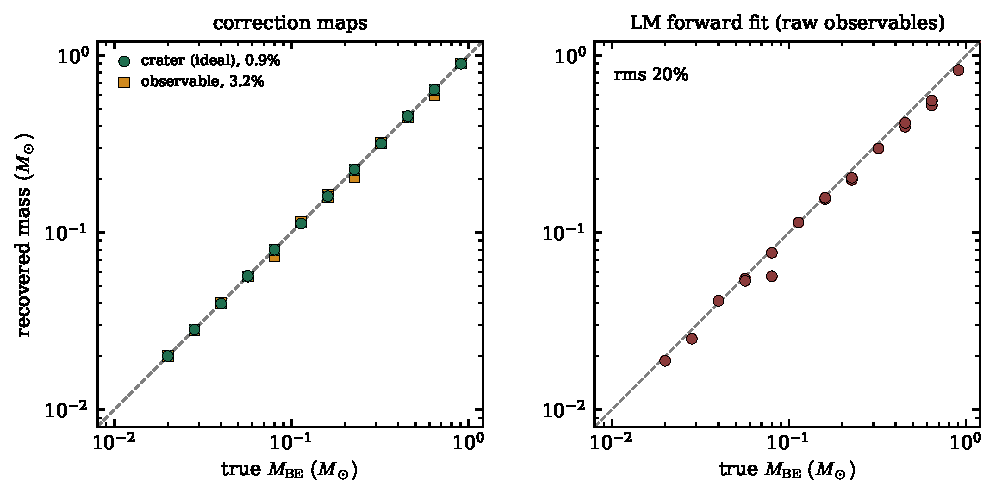
\includegraphics[width=\linewidth]{fig_fit_validation.pdf}
  \caption{Mass recovery tested on the 36 withheld subdivision (cell-center)
  models, using a correction built from the production grid only.
  \emph{Left:} the correction maps (recovered versus true $M_{\mathrm{BE}}$)
  -- the crater map (green, $0.95\%$ rms, the model-only ideal) and the
  operational map keyed on observable interpolated-background quantities
  $(M_{\mathrm{SED3bs}},\Scloud,\mathrm{FWHM})$ (orange, $3.2\%$) -- both lying
  on the 1:1 relation (dashed). \emph{Right:} the Levenberg--Marquardt forward
  fit of the raw center intensities and FWHMs scatters at $\sim$20\%,
  underestimating systematically, because the raw observables interpolate far
  less smoothly than the bias ratios.}
  \label{fig:fitval}
\end{figure}

\begin{figure}
  \centering
  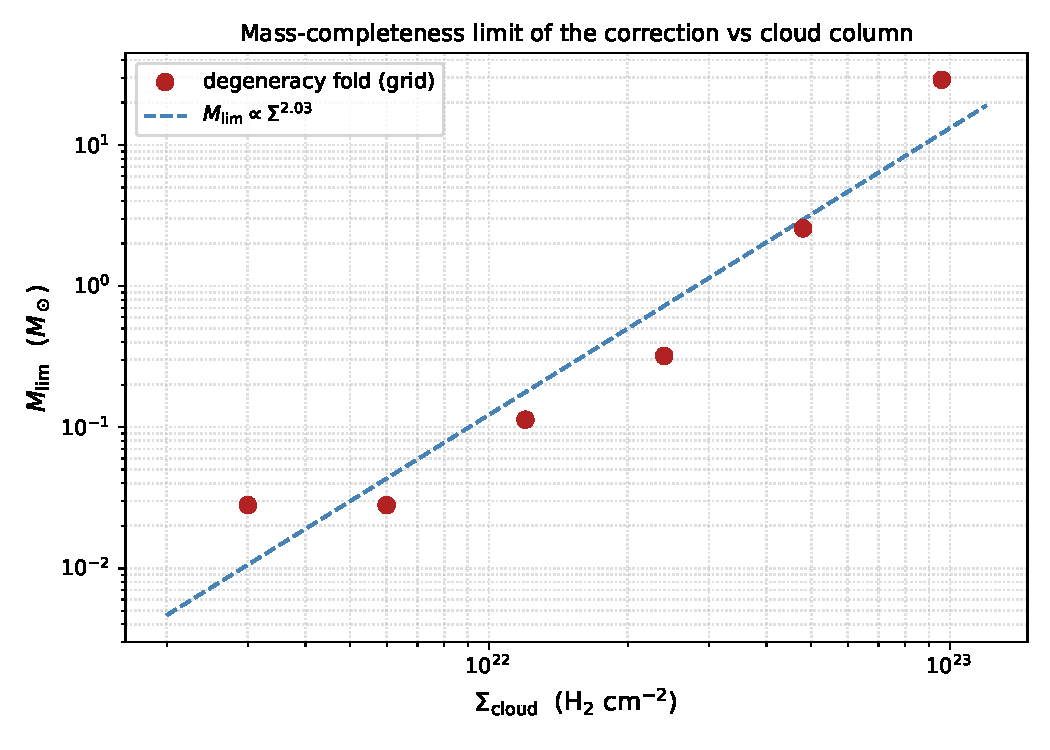
\includegraphics[width=\linewidth]{completeness_limit.pdf}
  \caption{Mass-completeness (degeneracy) limit of the correction as a
  function of cloud column. Points mark the grid mass at which the
  recoverable-mass$\,\rightarrow M_{\mathrm{BE}}$ mapping ceases to be
  monotonic; the dashed line is the near-quadratic scaling of
  Eq.~(\ref{eq:mlim}). Below this locus the correction is degenerate and is
  not applied.}
  \label{fig:mlim}
\end{figure}

\subsection{Mass floor and high-mass cap}
\label{sec:floorcap}

The low-mass floor ($\sim$0.01\,$\msun$ at the Aquila distance) is set by
the angular resolution: below the pixel, contrast and FWHM both saturate to
point-source-on-background and carry no recoverable size information, so the
grid cannot constrain such cores and does not attempt to. Per column, the
binding low-mass edge is whichever of this resolution floor or the
detectability limit (Sect.~\ref{sec:edge}) is the more restrictive.

The high-mass boundary is not a chosen cap but the intrinsic limit of the
pressure-truncated BE family. At each column the most massive constructible
core is the one whose truncation reaches the deep-concentration end of the
sequence; beyond it, no isothermal pressure-truncated sphere exists at that
mass and size. This boundary is therefore physically meaningful in a way a CMF
margin would not be: it is the largest mass a genuine single, cleanly measured
BE core can have at a given size, and it doubles as a diagnostic. A handful of
observed sources---$\sim$25 of the 685 Aquila cores, $\sim$4\%---lie above the
boundary, in the compact ($\mathrm{FWHM}\lesssim30''$), massive
($M\gtrsim1\,\msun$) corner. Reproducing them as BE spheres would require
$\ximax\sim70$--$150$, i.e.\ central-to-edge density contrasts far outside the
quasi-static isothermal regime and, indeed, outside any physically sensible
single-core structure. The natural interpretation is that these are not single
BE cores at all: at $260\,$pc a $\mathrm{FWHM}\lesssim30''$ aperture blends
multiple sources, and an interpolated background across such a source readily
sweeps in surrounding filament mass, inflating the apparent mass without a
commensurate increase in size and displacing the point up and to the left, out
of the BE locus. The grid boundary thus flags exactly the sources one would
want to treat separately---blended or background-contaminated---rather than
correct with a single-core template. We do not extend the grid to cover them:
doing so would mean fitting an unphysical BE profile to objects the model does
not describe. The method applies to the $\sim$96\% of cores consistent with
the BE family, and the boundary is stated as a domain of validity, not a
tuning choice.

\subsection{Geometry: a parsimonious template}
\label{sec:geometry}

We use spherical BE profiles rather than a richer non-spherical or
multi-parameter geometric family for a resolution reason: convolution to the
\emph{Herschel} beams washes out shape differences at the $\sim$5\% level, below
the noise, so geometric detail beyond a single concentration parameter is not
recoverable and would add unconstrained degrees of freedom. What the template
\emph{does} need is the freedom to reproduce the observed range of core sizes at
each mass, and this is where the earlier fixed-critical choice failed.

A direct comparison of model size against the published Aquila catalogue makes
the failure explicit. For a critical sphere at fixed temperature the mass and
radius scale together: from Eqs.~(\ref{eq:mass}) and (\ref{eq:r0}),
$M\propto\rhoc^{-1/2}$ and $\Rbe\propto\rhoc^{-1/2}$, so $M\propto\Rbe$. A more
massive critical sphere is therefore necessarily larger and more diffuse,
because its central density must fall to raise the mass, and the most massive
critical spheres in the grid reach $\sim$600$''$ where no observed core exceeds
$\sim$110$''$. Convolved to the catalogue resolution ($18.2''$, adding the
difference beam in quadrature to our $13.5''$ maps), the critical spheres match
observed sizes below $\sim$1\,$\msun$ but grow to a median model-to-observed
size ratio $\approx1.3$ over 1--10\,$\msun$, and about a fifth of the grid
occupied a size regime absent from the data. Real massive cores are compact and
centrally condensed, not large and diffuse; the fixed-critical family cannot
represent them.

The remedy, implemented here and described in
Sects.~\ref{sec:inversion}--\ref{sec:grid}, is to free the truncation $\ximax$
and parameterize each model by its observed mass and size. The stretch is a
property of holding $\ximax$ fixed, not of BE spheres as such. At fixed
temperature the critical family lies on $M\propto\Rbe$
($\mathrm{d}\log\Rbe/\mathrm{d}\log M = 1$), whereas the observed cores are
nearly flat ($\mathrm{d}\log\Rbe/\mathrm{d}\log M \approx 0.1$), that is, far
more centrally condensed than a critical sphere. Solving
Eq.~(\ref{eq:xiinvert}) for $\ximax$ at each observed $(M,\mathrm{FWHM})$ places
the model on the compact observed locus by construction: higher mass is then
reached by higher concentration (larger $\ximax$) rather than by inflation. The
reference extraction imposed a minimum measured size of $\sim$1.5 beams, so the
observed sizes near that floor are upper limits and the true concentration is,
if anything, slightly higher than the direct ratios imply.

The sub-critical, critical, and super-critical truncations are all physically
meaningful as core templates. The profile $\rho=\rhoc e^{-\psi}$ is a smooth,
monotone density distribution for any $\ximax$, and does not need to be a stable
equilibrium for the temperature bias and flux recovery to be representative;
real collapsing cores are not equilibria either. Physically the $\ximax$
sequence traces the prestellar sequence itself: weakly concentrated, pressure
confined, and often unbound at low $\ximax$; stable and increasingly self
gravitating up to the critical value; and collapsing above it, where the most
unambiguously prestellar (compact, massive) cores lie. The correction therefore
spans, and flags, this full sequence rather than assuming a single dynamical
state (Sect.~\ref{sec:grid}).

This parameterization is also what makes the four-observable correction well
posed. At fixed size the true mass varies by more than an order of magnitude as
$\ximax$ runs across its range, so size alone does not determine mass. The
degeneracy is broken by the recovered mass $M_{\mathrm{SED}}$, which scales
directly with $M_{\mathrm{BE}}$, and confirmed by the concentration, a monotone
function of $\ximax$ (Sect.~\ref{sec:concentration}). The mapping from the
measured tuple ($M_{\mathrm{SED}}$, $\Scloud$, source FWHM, concentration) to
true mass is thus single-valued, and none of the four observables is redundant:
dropping either the recovered mass or the concentration reopens the size--mass
degeneracy. This is the quantitative justification for the observable set of
Sect.~\ref{sec:observables}.

\subsection{Fixed $G_{0}$}
\label{sec:g0}

$G_{0}$ is held fixed because three-dimensional embedding makes a per-core
$G_{0}$ unrecoverable from the data, and because (Sect.~\ref{sec:tcalib})
the shielded cloud interior---which sets the core's heating environment---is
nearly $G_{0}$-insensitive at the relevant columns; the environmental
temperature variation is carried by $\Scloud$, not by $G_{0}$. The
calibration $G_{0}\approx 10$ is fixed by matching the high-resolution
SED-fit cloud temperature to the observed Aquila value.

\subsection{Interpolation accuracy}
\label{sec:interp}

Factor-2 node spacing is adequate where the observables vary smoothly, but
may be too coarse where an observable changes character: where the
70\,$\mu$m signed center intensity flips sign (cold cores in absorption) or
where a band transitions from optically thin to thick. We verify
interpolation by a hold-out test---comparing the interpolated observable
vector at a withheld node to a dedicated RT run---specifically at the nodes
bracketing those transitions, and refine locally if any observable exceeds a
few percent.

\begin{figure}[ht]
  \centering
  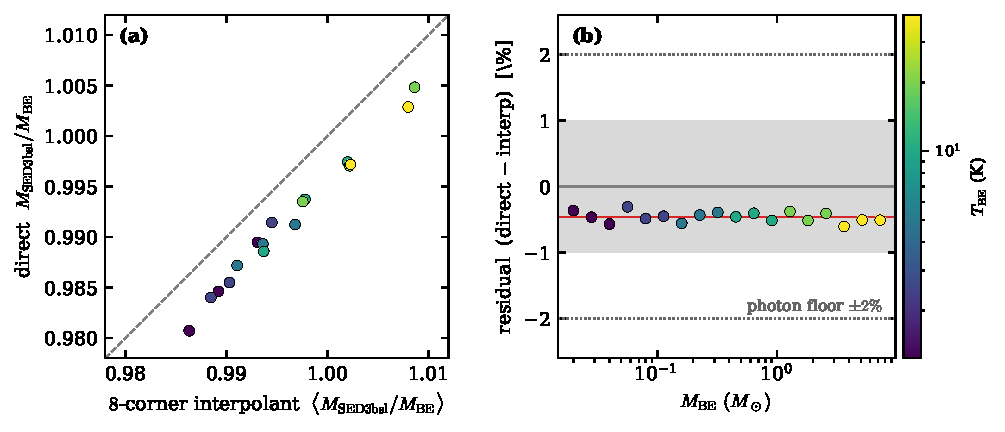
\includegraphics[width=\linewidth]{fig_gridconv.pdf}
  \caption{Grid-spacing convergence of the crater $\Phi_3$ mass bias.
  \emph{(a)} Directly computed bias $M_{\mathrm{SED3bsl}}/M_{\mathrm{BE}}$ at
  the 18 fully bracketed subdivision (cell-center) nodes versus the
  eight-corner linear interpolant; the dashed line is the 1:1 relation.
  \emph{(b)} The corresponding residual (direct minus interpolated, per cent)
  as a function of model mass; the shaded band is $\pm1\%$, the dotted lines
  mark the $\pm2\%$ photon-noise floor, and the red line is the mean.
  Points are colored by $\Tbe$. All residuals lie within $0.6\%$, confirming
  that the factor-2 production grid is adequate.}
  \label{fig:gridconv}
\end{figure}

\subsection{Dust-to-gas round-trip consistency}

The dust-to-gas mass ratio is $M_{\mathrm{dust}}/M_{\mathrm{gas}}$ (gas in
the denominator); the conversion of a total density to the dust density that
RADMC-3D requires uses the dust mass \emph{fraction}
$f = M_{\mathrm{dust}}/(M_{\mathrm{gas}}+M_{\mathrm{dust}}) = R/(1+R)$,
which differs from $R$ by $<1\%$. We adopt the same value
($R=0.01$, matching the published Aquila catalogue) in both directions:
to build $\rho_{\mathrm{dust}}$ and to convert recovered dust mass back to
total mass, and we use the same dust opacity $\kappa_\nu$ \citep{Ossenkopf+Henning1994}
in the RT and in the SED fit. The RT grid applies an opacity scaling factor
$\kappa_{\mathrm{scale}}=1.0746$ to the O\&H table, making it consistent with
the HGBS analytical approximation $\kappa_\nu=10\,(300\,\mu\mathrm{m}/\lambda)^{2}$\,
cm$^{2}$\,g$^{-1}$ used in Eq.~(\ref{eq:Iback}) to better than 0.5\% at all
\emph{Herschel} bands. Because the bias measurement is differential, the absolute calibration
(the choice of 0.01 versus the He-corrected dust-to-total-gas $1/141$)
cancels in the round trip and is a calibration footnote, not a source of
bias.

\subsection{Numerical hygiene retained}

We note the construction lessons that prevent recurrence of resolved bugs:
the central density must come from BE physics first
(Sect.~\ref{sec:inversion}); the inversion coefficient and the profile
builder must share one $m_{1}$; densities must be mass-conserving cell
averages, not point samples (Sect.~\ref{sec:massconserv}); a wall must sit
exactly at $\Rbe$ so no straddle cell exists and the BE/cloud assignment
loops use a single membership criterion (Sect.~\ref{sec:continuity}); and
artefact-contaminated models (BE edge density below cloud density) must not
be carried forward---the withdrawn factor-5 numbers
(Sect.~\ref{sec:cratervsinterp}) are an example.

% ======================================================================
\section{Direct comparison with the published Aquila catalogue}
\label{sec:konyves}
% ======================================================================

The Aquila catalogue of \citet{Konyves+2015} is the natural external test of
the correction. It was built from the same cloud with the same instrument,
but with a different extraction code (\emph{getsources} rather than
\emph{getsf}) and over the full $11\,\mathrm{deg^2}$ field rather than the
subfield used above, so it provides an independent sample an order of
magnitude larger. The two codes share the same interpolated-background
scheme, so their photometry is directly comparable. We take the published
core masses, dust temperatures and $\alpha_{\mathrm{BE}}$ from their Table~A.2
and the local background column $N_{\mathrm{back}}$, the peak contrast and the
core FWHM from their Table~A.1. Their column-density observables are measured
at $18.2''$ resolution against the $13.5''$ of the model grid; we therefore
deconvolve and reconvolve the sizes in quadrature and rescale the peak
contrast by $(\theta^2+18.2^2)/(\theta^2+13.5^2)$ before applying the
correction.

Two checks confirm that the published quantities are being reproduced
correctly. Fitting lognormals to the binned $\mathrm{d}N/\mathrm{d}\log M$
returns a peak of $0.62\,\msun$ for the robust prestellar sample, identical to
their quoted value, and $0.41\,\msun$ for the candidate sample against their
$0.34\,\msun$. Their prestellar selection is reproduced exactly by the
size-dependent criterion
$\alpha_{\mathrm{BE}}\le5\,(\mathrm{FWHM}/18.2'')^{-0.4}$, which recovers the
published classification for $100\%$ of the $685$ starless cores.

\subsection{The mass--size plane: the high-mass end is not made of single BE spheres}
\label{sec:masssize}

Figure~\ref{fig:masssize} places the published cores in the mass--size plane
of their Fig.~7 together with the model grid. The comparison is more
restrictive than the classical one against critical BE curves at fixed
temperature, because the grid is bounded not by a single analytic line but by
the whole pressure-truncated family as it is actually observed through the
beam. At the compact end the discrepancy is severe: among cores with
deconvolved sizes below $0.03$\,pc, $27$ have masses exceeding the largest
mass any BE sphere can present at that size, the most massive reaching
$11.5\,\msun$ against a family limit near $1.4\,\msun$. These objects are not
marginally outside the family; they lie an order of magnitude above it.

The same population is selected independently by the contrast ceiling of
Sect.~\ref{sec:ceiling}, which uses only the peak contrast and the local
background column and knows nothing about the mass or the size. Nineteen
cores lie above the ceiling, and they are the same compact, massive objects.
That two independent criteria -- one in the mass--size plane, one in the
contrast--column plane -- isolate the same sources is the strongest available
evidence that the high-mass end of the observed core population cannot be
interpreted as single isothermal BE spheres. Either the objects are
super-critical and already collapsing, or, as is likely for most of them at
the resolution of the survey, they are unresolved blends of several compact
sources. The fraction rises steeply with environment, from zero below
$6\times10^{21}\,\mathrm{cm^{-2}}$ to $39\%$ above
$2.4\times10^{22}\,\mathrm{cm^{-2}}$, which is where the crowding is worst.
This has a direct consequence for the interpretation of the CMF: the
high-mass tail, which carries the resemblance to the stellar IMF, is
precisely the part of the distribution least likely to consist of single
cores.

\subsection{The correction and the core mass function}
\label{sec:cmfcompare}

Applying the correction to the published prestellar sample gives a median
factor of $1.67$, with a strong environmental dependence: $1.37$ below
$6\times10^{21}\,\mathrm{cm^{-2}}$, $1.66$ between $6\times10^{21}$ and
$1.2\times10^{22}$, and $2.52$ above $1.2\times10^{22}\,\mathrm{cm^{-2}}$.
The integrated prestellar mass of the corrected sample rises by rather more
than a factor of two.

The effect on the shape of the CMF is larger than the effect on any single
mass. All power-law slopes quoted here are obtained by unbinned maximum
likelihood \citep{Clauset+2009}, working directly with the individual core
masses above a lower bound $M_{\mathrm{min}}$ selected by minimising the
Kolmogorov--Smirnov distance between the empirical and fitted cumulative
distributions; the standard error on the log-slope $\alpha$ is
$|\alpha-1|/\sqrt{n}$, with $n$ the number of cores above $M_{\mathrm{min}}$.
This avoids the bias and the inflated, ill-defined uncertainties that affect
least-squares fits to binned or cumulative counts, which matters here because
the high-mass tails contain few objects. Fitted this way over the corrected
prestellar cores, the high-mass slope of $\mathrm{d}N/\mathrm{d}\log M$ moves
from $-2.2\pm0.2$ before correction to $-1.9\pm0.2$ after it for the
\citet{Konyves+2015} sample, and the effect is stronger in the independent
\emph{getsf} extractions of the same field ($-2.9\pm0.3\rightarrow
-1.2\pm0.1$). In every case the distribution moves from one far steeper than
the stellar initial mass function to one consistent with, or approaching, the
Salpeter value of $-1.35$. The reason is structural
rather than statistical: the flux loss grows with background column, the
most massive cores sit preferentially in the densest filaments, and their
masses are therefore the most strongly underestimated. Correcting an
environment-dependent bias with an environment-dependent factor lifts the
high-mass end relative to the low-mass end and flattens the tail. A uniform
correction, however large, cannot do this.

\subsection{The physical scale of the correction's domain}
\label{sec:lowmass}

The preceding two subsections place a boundary near $2\,\msun$: no core above
that mass in the published catalogue is representable by a single
pressure-truncated BE sphere, and the entire high-mass tail of the observed
CMF consists of objects that lie outside the family. It is worth asking
whether that boundary is a property of our grid or a property of the physics.

The classical critical mass of a pressure-bounded isothermal sphere,
$M_{\mathrm{crit}}=1.18\,\cs^{4}G^{-3/2}P_{\mathrm{ext}}^{-1/2}$, provides the
answer independently of any grid. Evaluated over the range of conditions
relevant to prestellar cores it gives $1.2\,\msun$ at $10$\,K and
$n_{\mathrm{H_2}}=10^{4}\,\mathrm{cm^{-3}}$, $0.37\,\msun$ at
$10^{5}\,\mathrm{cm^{-3}}$, and $3.3\,\msun$ even at $20$\,K and
$10^{4}\,\mathrm{cm^{-3}}$. Thermal pressure therefore cannot support a
quasi-static core of more than a few solar masses anywhere in a molecular
cloud. A more massive object must be supported by turbulence or magnetic
fields, or else be dynamically collapsing; in either case it is not a member
of the family modelled here. The empirical boundary and the analytic one
agree, and they agree for a reason: the contrast ceiling of
Sect.~\ref{sec:ceiling} is the observational expression of the same limit on
central concentration that the critical mass expresses in terms of support.

This gives the domain of the correction a physical rather than a conventional
meaning. It applies to thermally supported cores, and the mass above which it
ceases to apply is set by the point at which thermal support fails, not by an
arbitrary cut. It is a coincidence worth noting that this boundary falls close
to the division between low- and intermediate-mass star formation. With the
customary core-to-star efficiency $\epsilon\simeq0.4$
\citep{Andre+2010,Konyves+2015}, a $2\,\msun$ core forms a star of
$\sim$$0.8\,\msun$, whereas the $10$--$20\,\msun$ cores that populate the
high-mass end of the Aquila CMF would form stars of $4$--$8\,\msun$, that is,
intermediate-mass rather than low-mass objects. The population to which the
present correction applies is thus, in stellar terms, the low-mass one, while
the objects it cannot treat are the progenitors of intermediate-mass stars
and are in any case not single thermally supported cores.

Two qualifications are needed. First, the upper mass limit of the model grid
itself is a construction parameter and not a physical boundary; it takes the
same value at every background column, which identifies it as such. The
physical statement rests on the analytic critical mass and on the observed
failure of the BE family to reach the required central concentration
(Sect.~\ref{sec:masssize}), not on the extent of the grid. Second, the
core-to-star efficiency is uncertain and probably environment-dependent, so
the mapping between the core boundary and the stellar mass range should be
read as indicative.

\subsection{Blending, and what the ceiling can and cannot establish}
\label{sec:blending}

The ceiling of Sect.~\ref{sec:ceiling} is a one-sided criterion. A contrast
above it demonstrates that the source is not a single pressure-truncated BE
sphere; a contrast below it shows only that the source is \emph{consistent}
with being one. Any extracted source may be a blend, including those that fall
inside the domain and are corrected, and it is worth stating plainly what the
present data can and cannot settle about this.

They cannot settle much, because every available test is blind in the regime
that matters. Source elongation, which the extraction limits to an axis ratio
of $\sim$2.5 and which reaches a median of only $1.46$ in the published
catalogue, carries no information about multiples separated by less than a
beam: a group of cores packed inside one beam is round, and for two components
of width $w$ separated by $d$ the induced axis ratio is
$\sqrt{1+(d/w)^{2}}$, which stays below $1.4$ for $d<w$. The above-ceiling
sources are in fact rounder than average (median axis ratio $1.32$ against
$1.47$), exactly as expected for strongly unresolved objects, so their shape
excludes nothing. Blend statistics estimated from source crowding are
circular, since an unresolved multiple enters the catalogue as a single
source and so cannot contribute to the measured surface density. And the
distribution of nearest-neighbour separations is truncated precisely at the
beam: no pair in the catalogue is closer than $18.2''$, while the sources are
strongly clustered on all scales that are measurable, exceeding the random
expectation by factors of $6$--$11$ between $18''$ and $73''$. The separation
distribution is thus rising steeply toward small scales exactly where the data
go blind, and the number of merged multiples is bounded from below but not
from above.

One test does discriminate, though only partially. Among the starless sources
that lie above the ceiling, the median $70\,\mu$m peak flux is negative and
only a quarter are positive, against roughly $60\%$ for the starless
population as a whole; these objects are seen in absorption against the warm
background rather than in emission. That argues against their harbouring an
undetected accretion luminosity, but a group of cold cores within one beam is
equally dark, so it does not distinguish a single concentrated object from an
unresolved cluster. Consistently, $28\%$ of the catalogued protostellar cores
lie above the ceiling, against $4\%$ of the prestellar and none of the
starless ones, confirming that the criterion responds to central concentration
of whatever origin.

It is therefore relevant that the correction degrades gracefully under
blending rather than failing. Applying the correction to synthetic
superpositions of two identical grid models, constructed by adding their
fluxes and broadening the profile in quadrature, returns between $0.81$ and
$0.88$ of the true combined mass for separations from zero to one beam, the
recovery improving as the pair separates. The blend presents nearly twice the
mass within nearly the same solid angle and therefore appears less affected by
flux loss than a single core of that total mass, so the correction applied is
somewhat too small. The comparison that matters, however, is with the
uncorrected value: the same blend retains only $\sim$$0.37$ of its true
combined mass before correction. A blended source is thus recovered to within
about $15\%$ of its total mass instead of being underestimated threefold, and
the residual error acts in the same direction as the correction itself, so
corrected masses remain lower limits.

The consequence for the interpretation of the CMF is the one that matters
most. If a significant share of the high-mass, high-column sources are
unresolved groups, then the high-mass tail of the observed CMF is built partly
from summed multiples and its resemblance to the stellar IMF is in part a
resolution effect. This possibility is not new \citep[][and references
therein]{Konyves+2015}, but the ceiling makes it quantitative and
source-by-source: the fraction of detections that cannot be single BE spheres
rises from zero below $6\times10^{21}\,\mathrm{cm^{-2}}$ to $41\%$ above
$2.4\times10^{22}\,\mathrm{cm^{-2}}$, which is where the massive cores are
found. Deciding between the available interpretations requires angular
resolution that Herschel does not provide, and interferometric follow-up of
the above-ceiling sources would be the natural test.

\subsection{Comparison with the earlier completeness simulation}
\label{sec:why25}

\citet{Konyves+2015} estimated the mass bias of their catalogue from a
Monte-Carlo experiment in which $5622$ synthetic cores were injected into the
Aquila maps and recovered through the same extraction chain. Their Fig.~B.2
gives a median ratio of derived to true mass of $\sim$$0.8$ above
$0.4\,\msun$ and $\sim$$0.7$ near the $0.2\,\msun$ completeness limit, with
the derived SED temperature exceeding the true mass-averaged dust temperature
by $\sim$$0.8$--$1$\,K. Both the extraction catalogue of that simulation and
its truth table are available, so the experiment can be re-analysed directly.

We first confirm that it is reproducible. Matching the $2101$ extracted
sources to the truth table by position identifies $1477$ recovered
injections, a recovery rate of $26\%$. Fitting modified-blackbody SEDs to
their $160$--$500\,\mu$m fluxes and binning by \emph{derived} mass, as in
their Fig.~B.2, returns a median mass ratio of $0.86$ above $0.4\,\msun$ and
$0.79$ near $0.2\,\msun$, with median temperature offsets of $+0.65$ and
$+1.26$\,K. These agree with the published values within the scatter, and
reproduce the trend that the deficit grows toward low derived mass. The
earlier estimate is therefore sound on its own terms, and the comparison
below is not a correction of an error but a difference of scope and
interpretation.

Expressed as the factor by which an observed mass must be multiplied, the
earlier experiment gives $1.25$ above $0.4\,\msun$ and $1.43$ near the
completeness limit, against the median $1.67$ obtained here for the real
prestellar cores. The two are closer than the quoted headline figures
suggest, and both agree that the bias increases toward lower mass; the
residual difference is some $30$--$40\%$, not the factor of two that a naive
comparison of a single quoted number with a single quoted number would imply.

Two properties of the earlier experiment differ from the present treatment
and are worth recording, since they bear on how such tests should be
designed. The first concerns the population that the test actually
calibrates. Taken as a whole, the injected sample is well matched to the
observations: all $5622$ models have a median contrast
$\mathcal{C}=(\mathrm{core}+\mathrm{bg})/\mathrm{bg}$ of $1.27$ on the
column-density map, close to the $1.33$ of the real starless cores. The
recovery, however, selects: only about a quarter of the models were
extracted, preferentially the brightest, and the recovered sample has a
median contrast of $1.83$ ($16$--$84\%$ range $1.52$--$2.84$). Its excess
column above the local background is thus a factor $2.5$ larger than that of
the real cores, an offset that persists at matched background column
(Fig.~\ref{fig:injcontrast}). A calibration derived from such a sample
describes a brighter population than the one to which it is applied. We note,
however, that within this simulation the recovered mass ratio is nearly
independent of contrast, so the offset alone does not account for the
residual difference in the correction factor.

The second concerns the background. The version of \emph{getsources} used
then determined source footprints less accurately than the present
\emph{getsf} implementation and tended to overestimate them. Where a core
sits on a declining background, an oversized footprint admits additional
flux from the background gradient, so that the interpolated background is
effectively under-subtracted. This is measurable in the same data: the
recovered $250\,\mu$m total fluxes exceed the true model fluxes by a median
of $19\%$, with the excess falling towards unity for the highest-contrast
sources, as expected if it originates in the background treatment rather
than in the sources themselves.

These two properties also indicate where the residual difference in the
correction factor originates. Three quantities have to be kept apart. The
grid's idealized ratio $M_{\mathrm{SED}}/M_{\mathrm{BE}}$, which carries the
temperature bias alone, has a median of $0.85$; its recoverable counterpart
$M_{\mathrm{SED}}^{\mathrm{rec}}/M_{\mathrm{BE}}$, which adds the modelled
flux loss, has a median of $0.37$; and the ratio measured in the earlier
simulation is $0.80$--$0.86$. The measured value agrees with the first and
not with the second: the recovered injections behaved as though they had lost
almost no flux. That is consistent with the background treatment described
above, since an extraction that adds $\sim$$19\%$ of flux through
under-subtraction beneath an oversized footprint will partly cancel a genuine
loss, leaving the temperature effect as the visible residual. On this reading
the agreement between the published ratio and the temperature-only prediction
is a coincidence of two competing errors rather than evidence that flux loss
is unimportant, and \citet{Konyves+2015} were correct to identify the
temperature effect as the dominant term \emph{for their extraction}, while a
more conservative footprint definition exposes the flux loss that their
background treatment had masked.

We emphasise that this reconciliation is inferred rather than demonstrated:
it rests on the measured $19\%$ flux excess and on the agreement of the
published ratio with the temperature-only prediction, but the two competing
terms have not been separated individually in that dataset. A decisive test
would be to re-extract the same injected field with \emph{getsf} and compare
the recovered fluxes directly, which we defer to future work. What can be
stated without qualification is that an injection test constrains only the
combined bias of a particular extraction, and not its decomposition into
temperature and flux-loss terms; the decomposition is accessible here only
because the models are radiative-transfer calculations with known intrinsic
masses and independently computed recoverable fractions.

These considerations motivate the design adopted here: model contrasts are
constructed to reproduce those of the extracted sources rather than to exceed
them, the detection floor is calibrated empirically on the observed lower
envelope of source peak against background column (Eq.~\ref{eq:floor}), and
the recoverable mass rather than the idealized model mass is used as the
interpolation coordinate. The general lesson is that an injection-recovery
test calibrates the bias for the population its \emph{recovered} sources
represent, which may differ appreciably from the population under study, and
that such a test constrains only the combined bias and not its decomposition
into temperature and flux-loss terms.

\begin{figure}
  \centering
  \includegraphics[width=\linewidth]{fig_injected_vs_real_contrast}
  \caption{Contrast $(\mathrm{core}+\mathrm{bg})/\mathrm{bg}$ of the model
  sources injected into the Aquila field for the earlier completeness
  simulation, compared with the real starless cores of
  \citet{Konyves+2015}. \emph{Left:} the full injected population (grey) has
  a contrast distribution close to that of the real cores, but the subset
  actually recovered by the extraction (red) is shifted to markedly higher
  contrast, with a median of $1.83$ against $1.33$. \emph{Right:} the same
  comparison against local background column, with binned medians; the
  offset persists at matched column and is therefore not an environmental
  effect. The recovered sample therefore
  represents a brighter population than the one to which the resulting
  calibration was applied, although within this simulation the recovered mass
  ratio itself depends only weakly on contrast.}
  \label{fig:injcontrast}
\end{figure}

\begin{figure}
  \centering
  \includegraphics[width=\linewidth]{fig_mass_size_konyves}
  \caption{Mass--size diagram for the starless cores of
  \citet{Konyves+2015}, compared with the pressure-truncated BE model grid
  (grey points). Filled and open triangles are their prestellar and other
  starless cores; the solid curves are critical BE spheres at $7$ and
  $20$\,K, as in their Fig.~7. Circled sources lie above the observable
  contrast ceiling of Sect.~\ref{sec:ceiling} and cannot be single BE
  spheres. Below $0.03$\,pc a substantial population lies far above the
  largest mass the BE family can present at that size, reaching
  $11.5\,\msun$ against a family limit near $1.4\,\msun$.}
  \label{fig:masssize}
\end{figure}

% ======================================================================
\section{Universality: application to seven clouds}
\label{sec:multicloud}

The corrector adopted here is expressed entirely in distance-invariant
observables: the recoverable mass, the local background column, and the
peak-to-mean surface brightness within the footprint
(Sect.~\ref{sec:invariant}). No angular size, and hence no size deconvolution
and no distance, enters the interpolation. This makes it
possible to apply the identical operation to clouds at very different
distances and to ask whether the inferred correction is a property of the
sources or of the observation. We have done this for seven regions extracted
uniformly with \emph{getsf}: Scorpius ($130$\,pc), Ophiuchus ($144$\,pc),
Aquila ($260$\,pc), Orion~A ($432$\,pc), California ($470$\,pc), Cygnus~X
($1150$\,pc), and the W3/W4/W5 complex ($1700$\,pc). The distance adopted for the last of these is
an inverse-variance weighted mean of twelve determinations across the complex
(individual values $1451$--$2184$\,pc), giving $1706\pm44$\,pc; the complex is
extended along the line of sight, so this complex-wide value is somewhat
smaller than the maser-parallax distance to W3 itself \citep[$\sim$$2$\,kpc;
][]{Xu+2006}.

The raw median correction factor varies from cloud to cloud, but almost all of
that variation is a sampling effect: a nearer cloud resolves fainter, less
massive cores that lie closer to the detection floor, where the correction is
largest, so its median is pulled up. Compared over a fixed mass interval,
$0.1$--$2\,\msun$, the factors collapse onto a narrow range. Scorpius gives
$1.51$, Aquila $1.55$, Orion~A $1.51$, California $1.37$, Cygnus~X $1.60$, and
W3/W4/W5 $1.37$, that is, $1.4$--$1.6$ across a factor of thirteen in distance
(Fig.~\ref{fig:sixcloud}a). The correction is, to within its scatter,
independent of distance. That it takes the same value at $1700$\,pc as at
$130$\,pc, with no distance information used at any stage, is the strongest
evidence we can offer that it captures a physical property of the cores and
their measurement rather than an artefact of any one field.

Ophiuchus is the single exception, at $2.37$ in the same mass interval. This
is not a distance effect --- Scorpius, at essentially the same distance,
follows the general trend --- but an environmental one. The L1688 ridge is
denser and more strongly illuminated by the neighbouring OB stars of
Sco~OB2 than the other fields, and both a higher background and a stronger
radiation field increase the flux lost outside the measured footprint that the
correction compensates. A larger factor for cores of the same mass is
therefore expected, and is consistent with the environmental dependence seen
within every cloud individually (Sect.~\ref{sec:cmfcompare}).

The effect on the core mass function is likewise reproduced in every cloud.
Fitted by unbinned maximum likelihood (Sect.~\ref{sec:cmfcompare}), the
high-mass slope moves from the steep published values, which range from
$-2.0$ to $-6.3$, to corrected values between $-1.0$ and $-2.4$, in every case
towards or beyond the Salpeter slope of $-1.35$ (Fig.~\ref{fig:sixcloud}b).
The published slopes scatter widely; the corrected ones do not.

\subsection{A shallow corrected CMF, and a possible link to ALMA-IMF}
\label{sec:shallowcmf}
\note{HYPOTHESIS --- promising but not yet established; flagged here so it is
not lost, and a candidate headline for a follow-up paper once the injection
test below confirms or refutes it.}

Among the four best-resolved clouds --- Scorpius, Ophiuchus, Aquila, and
California, all with beams below $0.03$\,pc --- the corrected high-mass slope
is consistently \emph{shallower} than Salpeter, not merely flattened towards
it: $-1.19\pm0.37$, $-1.04\pm0.09$, $-1.23\pm0.09$, and $-1.05\pm0.08$
respectively. Combined into a single distribution ($334$ corrected cores above
the KS-selected $M_{\mathrm{min}}=0.65\,\msun$), they give $-1.18\pm0.06$,
which departs from the Salpeter value of $-1.35$ at about $3\sigma$ and lies
between it and the top-heavy slopes of $\alpha\simeq-0.9$ to $-1.0$ that the
ALMA-IMF programme reports for distant massive protoclusters
\citep[e.g.][]{Motte+2018}.

The potential significance is that these two lines of evidence approach the
same conclusion from opposite regimes. ALMA-IMF measures top-heavy core mass
functions in distant, high-mass, blend-prone regions and must contend with the
question of whether the shallowness is intrinsic or an effect of resolution and
environment. The clouds here are nearby, low-mass, and well resolved, and their
published mass functions were consistent with the stellar IMF; it is only after
the removal of the temperature-and-flux-loss bias that they, too, become
shallower than Salpeter. If a resolved, low-mass sample and an unresolved,
high-mass one independently favour a shallow CMF, the shallowness is more
plausibly a property of dense-core populations than an artefact of either
method.

This must be stated as a hypothesis, not a result, because of an alternative
that the present data cannot yet exclude: the correction is
environment-dependent and lifts the high-mass end more than the low-mass end,
so in principle it could tilt an intrinsically Salpeter distribution to a
shallower one by construction. The accuracy validation
(Sect.~\ref{sec:accuracy}) shows the correction recovers true masses rather
than inflating them arbitrarily, which argues against a purely artefactual
tilt, but it does not by itself prove that an input slope is preserved. The
decisive test is direct and is already required for other reasons
(Sect.~\ref{sec:multicloud}, and the injection programme noted in
Sect.~\ref{sec:accuracy}): inject a synthetic core population with a known
input slope --- Salpeter, and separately a shallower and a steeper value ---
into the real maps, carry it through extraction and correction, and verify that
the recovered slope matches the input. If a Salpeter input is returned as
Salpeter, then the shallow slope recovered from the real clouds is a property
of the cores; if a Salpeter input is returned as shallow, the effect is
manufactured and must be removed. Until that test is done, the number
$-1.18\pm0.06$ should be read as a motivated hypothesis with $3\sigma$
support and an independent counterpart in the ALMA-IMF results, and not as an
established measurement.

The two high-mass regions, Cygnus~X and W3/W4/W5, behave alike and differently
from the nearby low-mass clouds in one instructive respect. Both contain
genuinely massive cores, and for these the correction is much larger than the
$\sim$$1.5$ found at low mass: in Cygnus~X the median factor rises from $1.6$
over $0.1$--$2\,\msun$ to $2.6$ over $1$--$10\,\msun$ and $3.1$ over
$2$--$20\,\msun$. Taken at face value this shifts the most massive apparent
cores from $2$--$20$ to $6$--$60\,\msun$, which would make Cygnus~X look like
the massive-core reservoir a high-mass star-forming region is expected to be.
We are deliberately cautious about this reading. At $1150$--$1700$\,pc a single
beam spans $0.2$--$0.3$\,pc, and the most massive ``cores'' in these regions
are, on the evidence of higher-resolution studies elsewhere
(Sect.~\ref{sec:blending}; \citealt{Motte+2018}), predominantly unresolved
clusters. A large upward correction applied to a blended system does not
recover the mass of a single object; it returns the mass of the equivalent
single core that would reproduce the blend's observables, which for a true
multiple exceeds any of its members. The steepness of the corrected Cygnus~X
slope ($-3.9$), which does not flatten to Salpeter as the resolved nearby
clouds do, is consistent with this: the high-mass end is built from summed
multiples whose individual members are not accessible to \emph{Herschel}. The
factor of three is therefore best read as a statement about the flux missed by
the extraction, not as a claim that individual $60\,\msun$ prestellar cores are
present. Interferometric follow-up is the only way to convert these blended
masses into a resolved high-mass CMF.

\begin{figure}
  \centering
  \includegraphics[width=\linewidth]{fig_sixcloud_universality}
  \caption{The distance-invariant correction applied to seven clouds spanning
  $130$--$1700$\,pc. \emph{Left:} the median correction factor over a fixed
  $0.1$--$2\,\msun$ interval as a function of distance; six of the seven clouds
  lie in the shaded band $1.37$--$1.60$ with no trend in distance, and
  Ophiuchus (red) is a denser, more strongly illuminated environment.
  \emph{Right:} maximum-likelihood high-mass CMF slopes before (grey) and
  after (red) correction; the published slopes scatter from $-2$ to $-6$,
  the corrected ones cluster near the Salpeter value (dotted).}
  \label{fig:sixcloud}
\end{figure}

Two caveats apply specifically to the most distant regions and are important
for interpreting them. First, coverage falls with distance: at $1700$\,pc most
sources are unresolved and fall outside the model hull, so only $12\%$ of the
W3/W4/W5 sources are corrected, against $50$--$70\%$ in the nearest clouds, and
the corrected slopes there rest on fewer objects. Second, and more
fundamentally, a single beam at $1700$\,pc subtends $\sim$$0.3$\,pc, so many
catalogued ``cores'' in W3/W4/W5 are almost certainly unresolved clusters
rather than single objects. This is a generic feature of distant high-mass
regions: wherever \emph{Herschel}-scale cores in such regions have been
re-observed at the far higher resolution of ALMA, they fragment into clusters
of many objects. In the W43-MM1 ridge --- a different and still more distant
mini-starburst at $5.5$\,kpc, cited here only as an illustration --- ALMA
resolves the clump into $131$ cores \citep{Motte+2018}. There is every reason
to expect the same in W3/W4/W5 at $1700$\,pc. The masses we correct there are
therefore those of the blended systems, not of their members, and the
still-steep corrected slope ($-2.4$) partly reflects this, the tail being built
from summed multiples. A distant high-mass region is thus a test of whether the
method \emph{breaks} --- it does not --- rather than a clean measurement of a
resolved core population.

Finally, we note that our source lists are those of the uniform \emph{getsf}
extractions and have not been cleaned of contamination by field stars or
background galaxies unassociated with each cloud, a step commonly taken in
dedicated single-cloud studies. This contamination is expected to be a minor
and roughly distance-independent additive component, and it cannot produce the
systematic, environment-dependent trends we recover; but it is a further reason
to read the individual high-mass slopes as indicative rather than definitive.

\section{Summary and next steps}
% ======================================================================

We have defined a per-core RT forward-modeling method that corrects the two
compounding biases in \emph{Herschel} SED-derived prestellar core masses---
the temperature-gradient warm bias and the interpolated-background
over-subtraction flux loss---and delivers a quantitative bias-vs-(mass,
column) surface. The model family is the critical BE sphere, built with
analytically derived central densities, mass-conserving discretization, a
wall snapped to $\Rbe$, and a detectability-limited low-mass edge; the
embedding cloud is sized to the convolved core scale with the cloud surface
density $\Scloud$ as the physical third axis. Calibration places the field
at $G_{0}\approx 10$, matched SED-to-SED to the observed Aquila temperatures.
A demonstration at $0.1\,\msun$ confirms a $\sim$1.5 mass under-estimate from
interpolated background subtraction, corrected by the crater scheme.

Two further results constrain and validate the method. First, the four-band
SED fit collapses at $\Scloud\approx2.4\times10^{22}\,\mathrm{cm^{-2}}$
where the background-subtracted 160\,$\mu$m flux crosses zero; the
three-band (250--500\,$\mu$m) fit is unaffected. A field-independent
criterion -- use $M_{\mathrm{SED3}}$ when $M_{\mathrm{SED4}}/M_{\mathrm{SED3}}>1.3$
(Sect.~\ref{sec:bandselect}) -- recovers the clean masses with no cloud-specific
noise model required. Second, the grid reproduces the HGBS
confusion-completeness model and its first-order mass and temperature bias
(Sect.~\ref{sec:completeness}), an external validation against published
results. A known-truth injection test (Sect.~\ref{sec:injtest}) localises
the remaining error to source/background separation quality rather than the
temperature modeling.

Remaining steps:
(1)~complete the production $(\Scloud,\Tbe,\rhoc)$ grid with the corrected
runs and verify continuity and mass conservation across it;
(2)~map both biases as functions of mass and column---the quantitative core
of the paper;
(3)~confirm the observed column range maps to the observed cloud-temperature
range at $G_{0}\approx 10$, and that embedded model cores span the observed
core SED-temperature range;
(4)~build the fitting pipeline (grid loader, scattered interpolator,
residual function, bounded LM) on the final catalogue, selecting
$M_{\mathrm{SED3}}$ or $M_{\mathrm{SED4}}$ via Eq.~(\ref{eq:sedselect});
(5)~improve the source/background separation under the core
(lower-envelope/\texttt{getimages}-style background; per-source deblended
images), the dominant remaining error (Sect.~\ref{sec:injtest});
(6)~run the non-uniform-cloud sensitivity test (Sect.~\ref{sec:uniformcloud})
to budget the idealization;
(7)~apply to Aquila and, in a companion paper, to additional clouds.

% ----------------------------------------------------------------------
\bibliographystyle{plainnat}  % switch to aa.bst for A&A submission
\bibliography{rt_mass_correction}

% ======================================================================
% PROJECT NOTES --- NOT FOR SUBMISSION
% This appendix is an internal working record of decisions and strategy
% that are NOT part of the method itself. It exists so that the rationale
% behind structural choices survives across working sessions, and as a
% place to accumulate further non-method decisions over time. Strip the
% whole appendix before submitting any version of the paper(s).
% ======================================================================
\clearpage
\appendix

\section{Per-field diagnostics}
\label{app:fields}

Figures~\ref{fig:mfwhm} and \ref{fig:contrast} collect two diagnostics across
the seven fields, obtained with a common reader that locates catalogue columns
by header name and identifies the $13.5''$ H$_2$ column-density band by its
unit string rather than by an assumed index. The latter matters because the
band numbering is not uniform: the surfdens map is band~02 in most catalogues
but band~03 in California and Cygnus~X, where a sub-$160\,\mu$m band shifts the
numbering.

\begin{figure*}
  \centering
  \includegraphics[width=\textwidth]{fig_mfwhm_allfields}
  \caption{Core mass against beam-subtracted physical FWHM for each field
  (grey), with the detectable model-grid nodes overplotted (red, $M_{\rm BE}$).
  The sources track the grid locus, confirming that the correction interpolates
  within the sampled region rather than extrapolating. The fields shift
  systematically along the sequence with distance: the nearest clouds populate
  the compact, low-mass corner, the most distant reach larger sizes and higher
  masses.}
  \label{fig:mfwhm}
\end{figure*}

\begin{figure*}
  \centering
  \includegraphics[width=\textwidth]{fig_contrast_allfields}
  \caption{Distributions of source contrast
  $(\mathrm{core}+\mathrm{bg})/\mathrm{bg}$ (left) and their median and
  interquartile range against distance (right). The distributions overlap
  closely and show no trend with distance. Because contrast is a ratio of
  intensities in the same map, and hence distance-invariant, this flatness is a
  consistency check that the cross-field comparison is methodologically sound.
  Ophiuchus has the lowest median contrast, consistent with its being the
  densest field.}
  \label{fig:contrast}
\end{figure*}

A feature of Fig.~\ref{fig:mfwhm} worth noting is the population of sources
lying \emph{below} the lower envelope of the grid in the two nearest clouds:
$65\%$ of Scorpius and $61\%$ of Ophiuchus sources fall below the minimum-mass
BE line at their measured size, against $\sim$$9\%$ in the mid-distance clouds
and essentially none in the most distant. These are not artefacts. The grid's
lower envelope is the least-massive self-gravitating BE sphere at a given
radius (the $\rho_{\mathrm{edge}}\ge\rho_{\mathrm{cloud}}$ condition); a source
below it has the size of a core but less than the mass such a core requires,
and is therefore a diffuse, probably unbound condensation rather than a
prestellar core. Their median masses are a few thousandths of a solar mass in
the nearest clouds, rising with distance ($0.003\,\msun$ at $130$\,pc to
$0.05\,\msun$ at $1700$\,pc) in step with the surface-brightness sensitivity
limit. They appear only nearby because only there does the sensitivity reach
such small masses: a fixed physical density enhancement subtends a smaller
solid angle with increasing distance, so the beam progressively dilutes its
peak surface brightness against the surrounding background until it drops below
the detection threshold. The distant clouds contain the same condensations,
but beam dilution renders them invisible. Most ($74$--$87\%$) are resolved,
arguing that they are real low-mass structures rather than noise peaks. The correction leaves them
untouched --- they lie outside the model hull and receive no BE mass --- which
is the correct behaviour, since they are not BE cores. The low nominal coverage
in the nearest clouds is thus largely the method declining to correct objects
that are not cores, not a failure to correct those that are.

\section*{Project notes (internal --- not for submission)}
\addcontentsline{toc}{section}{Project notes}
\refstepcounter{section}

\subsection*{N.1 \quad Publication strategy and page budget}

\paragraph{Constraint.} A\&A allows $\sim$12 pages plus $\sim$5 appendix
pages free of charge. The full superset draft exceeds this because it does
two jobs at once: a \emph{method specification} (every construction detail
and caution) and a \emph{paper} (the argued case for a reader). These have
different audiences, so the resolution is to separate ``what a referee needs
to evaluate the result'' from ``what is needed to reproduce it,'' pushing
the latter into appendices or a companion.

\paragraph{Option A --- single $\sim$12-page methods paper, details pruned.}
Most of what reads as detail to a general reader is numerical hygiene
(analytic central density, the $m_{1}/\sqrt{4\pi}$ coefficient,
mass-conserving cells, the wall at $\Rbe$, the telescoping proof). A referee
needs to know these were done correctly, not see the derivations: compress
to a few sentences in the main text with the equations and verification in
an appendix. The discussion (bias-vs-environment framing, validity
reasoning) stays in full---it is the contribution, not detail.

\paragraph{Option B --- two papers (preferred).} Split as in the filament
trio template:
\begin{itemize}
  \item \textbf{Paper~I (method).} BE construction, RT calibration, the two
        bias mechanisms, crater-vs-interpolated, the forward-model-and-fit
        framework, and all validity points; demonstrated on a single
        illustrative core or a minimal grid, with no Aquila CMF claims.
        Heavy numerics ($m_{1}$, mass conservation, discretization) in an
        appendix.
  \item \textbf{Paper~II (Aquila application).} The calibrated method
        applied to the full Aquila catalogue: the bias-vs-(mass, column)
        surface and corrected masses.
  \item \textbf{Companion (seven clouds).} As planned; may be longer.
\end{itemize}

\paragraph{Why the split is preferred (beyond page count).}
(i)~The method is genuinely separable: the validity arguments (uniform
cloud, the edge, second-order corrections, comparison-to-standard) are about
the method and are strongest stated once, cleanly, without Aquila results
competing for space. (ii)~Citation dynamics: a clean method paper is more
adoptable and more citable than a hybrid, and establishes the framework for
others before the application lands---consistent with the programme's
``methodologically grounded scepticism is underprovisioned'' framing.
(iii)~Schedule de-risking: the method paper can go out once the grid is
built and the demonstration closes, independent of finishing the full Aquila
bias surface (the longer pole). Cost: the usual two-paper overhead (two
introductions, some repeated setup, and Paper~I needs \emph{enough}
application to convince).

\paragraph{Tentative partition of the current superset.}
Sections~1--3 and Discussion~4.1, 4.5--4.9 $\rightarrow$ Paper~I, with the
heavy numerics in Paper~I's appendix. The \emph{core} of the uniform-cloud
argument (4.2) is a method-validity point and stays in Paper~I; the
Aquila-specific edge mapping and floor/cap (4.3--4.4) defer to Paper~II.
The bias surface, corrected catalogue, and CMF implications $\rightarrow$
Paper~II. \note{Decide the final partition once results are in: if the bias
surface is compact, a single pruned paper may still fit; if rich, the split
is forced. Keep this superset as the complete record and tag section headers
with their destination (Paper~I / Paper~II) when we commit.}

\subsection*{N.2 \quad (reserved for further non-method decisions)}

\note{Placeholder. Add here, with dates, any later decisions that should
survive across sessions but do not belong in the method text---e.g.\ changes
to the publication plan, collaborator/division-of-labour decisions, target
journals, scope changes, or strategic framing choices.}

\end{document}
